%Plantilla basada en "Template for Masters / Doctoral Thesis" (plantilla disponible en writeLaTex) que subió LaTeXTemplates.com

\documentclass[11pt]{book}
\usepackage[paperwidth=17cm, paperheight=22.5cm, bottom=2.5cm, right=2.5cm]{geometry}
\usepackage{amssymb,amsmath,amsthm} %paquete para símbolo matemáticos
\usepackage[spanish]{babel}
\usepackage[utf8]{inputenc} %Paquete para escribir acentos y otros símbolos directamente
\usepackage{enumerate}
\usepackage{graphicx}
\usepackage{mathrsfs}
\usepackage{verbatim}
\usepackage{cite}
\usepackage{subcaption} %Subfiguras
\usepackage{verbatim}
\graphicspath{{Img/}} %En qué carpeta están las imágenes
\usepackage[nottoc]{tocbibind}
\usepackage[pdftex,
            pdfauthor={NOMBRE DEL AUTOR},
            pdftitle={Tesis Amadio Camilo},
            pdfsubject={ÁREA DE LA TESIS},
            pdfkeywords={PALABRAS CLAVE},
            pdfproducer={Latex con hyperref},
            pdfcreator={pdflatex}]{hyperref}
\usepackage{amssymb}


\usepackage[dvipsnames]{xcolor}
%\newcommand{\r}[1]{\textcolor{red}{#1}}
\def\red{\color{red}}
\def\magenta{\color{magenta}}

%\includeonly{Capitulos/cap3}

\begin{document}

%----------------------------------------------------------------------------------------
%	COMANDOS PERSONALIZADOS
%----------------------------------------------------------------------------------------

%SI TU TESIS TIENE TEOREMAS Y DEMOSTRACIONES, PUEDES DESCOMENTAR Y USAR LOS SIGUIENTES COMANDOS

%\renewcommand{\proofname}{Demostración}
%\providecommand{\norm}[1]{\lVert#1\rVert} %Provee el comando para producir una norma.
%\providecommand{\innp}[1]{\langle#1\rangle} 
%\newcommand{\seno}{\mathrm{sen}}
%\newcommand{\diff}{\mathrm{d}}

%\newtheorem{teo}{Teorema}[section] 
%\newtheorem{cor}[teo]{Corolario}
%\newtheorem{lem}[teo]{Lema}

%\theoremstyle{definition}
%\newtheorem{dfn}[teo]{Definición}

%\theoremstyle{remark}
%\newtheorem{obs}[teo]{Observación}

%\allowdisplaybreaks


%----------------------------------------------------------------------------------------
%	PORTADA
%----------------------------------------------------------------------------------------

\title{Tesis Amadio Camilo Leonel} %Con este nombre se guardará el proyecto en writeLaTex

\begin{titlepage}
\begin{center}

\textsc{\Large Universidad Nacional de La Plata}\\[4em]

%Figura
\begin{figure}[h]
\begin{center}

\includegraphics[width=5 cm]{Escudo.jpg}
\end{center}
\end{figure}

\vspace{1em}

\textsc{\huge \textbf{
Funciones Espectrales \\[2mm]
En Teorías Cuánticas De Campos \\[2mm]
Con Singularidades
}}\\[4em]

\textsc{\large Trabajo de Diploma}\\[1em]

\textsc{Para obtener el Título de }\\[1em]

\textsc{Licenciado en Física}\\[1em]

\textsc{presenta}\\[1em]

\textsc{\Large Camilo Leonel Amadio}\\[1em]

\textsc{\large Director: Pablo Pisani}

\end{center}

\vspace*{\fill}
\textsc{La Plata, Argentina \hspace*{\fill} 2019}

\end{titlepage}

\begin{comment}
%----------------------------------------------------------------------------------------
%	DECLARACIÓN
%----------------------------------------------------------------------------------------

\thispagestyle{empty}
\vspace*{\fill}
\begingroup
``Con fundamento en los artículos 21 y 27 de la Ley Federal del Derecho de Autor y como titular de los derechos moral y patrimonial de la obra titulada ``\textbf{TÍTULO DE LA TESIS}'', otorgo de manera gratuita y permanente al Instituto Tecnológico Autónomo de México y a la Biblioteca Raúl Bailléres Jr., la autorización para que fijen la obra en cualquier medio, incluido el electrónico, y la divulguen entre sus usuarios, profesores, estudiantes o terceras personas, sin que pueda percibir por tal divulgación una contraprestación''.

\centering

\hspace{3em}

\textsc{AUTOR}

\vspace{5em}

\rule[1em]{20em}{0.5pt} % Línea para la fecha

\textsc{Fecha}
 
\vspace{8em}

\rule[1em]{20em}{0.5pt} % Línea para la firma

\textsc{Firma}

\endgroup
\vspace*{\fill}



%----------------------------------------------------------------------------------------
%	DEDICATORIA
%----------------------------------------------------------------------------------------

\pagestyle{empty}
\frontmatter

\chapter*{}
\begin{flushright}
\textit{DEDICATORIA}
\end{flushright}

\end{comment}

%----------------------------------------------------------------------------------------
%	AGRADECIMIENTOS
%----------------------------------------------------------------------------------------

\chapter*{Agradecimientos}
%\markboth{AGRADECIMIENTOS23}{AGRADECIMIENTOS} % encabezado 

Me gustan los agradecimientos cortos, y la birra fría.

\begin{enumerate}
    \item A Mama que me demostró cual es el camino hoy y cada día de mi vida, con el ejemplo y no solo con palabras
    \item papa 
    \item  A mis tíos y tías que siempre me extendieron una mano cuando la necesite
    \item A Mi Abue Mirtha, todo esto te lo dedico a vos, que siempre estuviste 
    \item A  todos mis amigos que me acompañaron a lo largo de estos años, sin ellos me hubiera vuelto a las 2 semanas 
    \item A Wikipedia y Julioprofe
    \item Al Rasta, Lolo y el Diquin, que me acompañaron a salir de joda 
    \item A mis mejores amigos, Lucas, La Sol y la Celia
    \item A la cervecería Quilmes que sin ella probablemente ya me hubiera suicidado hace mucho
    \item A Ana y Analia, que son las mejores bibliotecarias que existen, no me imagino como hubiera sido sin ellas. 
\end{enumerate}



%----------------------------------------------------------------------------------------
%	PREFACIO
%----------------------------------------------------------------------------------------

\chapter*{Prefacio}

\pagestyle{plain}
\markboth{PREFACIO23}{PREFACIO} % encabezado 

 En el año 2002 en un trabajo realizado por H. Falomir, P.A.G. Pisani y M.A. Muschietti  \cite{doi:10.1063/1.1809257} se estudiaron la resolvente y extenciones autoadjuntas de operadores singulares de la forma $A = - \partial ^2 _x + g(g-1) x ^{-2}$ en un intervalo unidimensaional compacto, encontrando que la {\it función-$\zeta$} posee polos simples en $s _n = - \left( g - \frac{1}{2} \right) n$ donde $n \in \mathbb{N} _+$. Lo cual se aparta del comportamiento esperado para el caso regular en el cual $\zeta (s)$ poseería polos simples en $s _n = \frac{1 - n}{2}$ con  $n \in \mathbb{N} _+$.

En este trabajo de tesis se estudió la {\it función-$\zeta$} del operador ${A = - \partial ^2 _x + \frac{\alpha}{x}}$ en el intervalo compacto $[0,L]$ encontrando que tal como ocurre en el caso regular los polos se ubican según $s _n = \frac{1 - n}{2}$, pero a diferencia de este la singularidad conduce a la aparición de un polo doble, lo cual implica que el desarrollo del {\it heat-kernel} posee términos logaritmicos. Tal como se conjeturó en 1980 por Constantine Callias y Clifford H. Taubes \cite{callias1980}.



%----------------------------------------------------------------------------------------
%	TABLA DE CONTENIDOS
%---------------------------------------------------------------------------------------

\tableofcontents


%----------------------------------------------------------------------------------------
%	TESIS
%----------------------------------------------------------------------------------------
\mainmatter %empieza la numeración de las páginas
\pagestyle{headings}

%  Incluye los capítulos en el folder de capítulos

\chapter{Introducción}


En Teoría Cuántica de Campos el cálculo de ciertas magnitudes físicas (acciones efectivas, energías de vacío, amplitudes de dispersión, etc.) conduce, en general, a valores formalmente divergentes, por lo cual se requiere un método para extraer resultados finitos. 

En el presente capítulo se presentarán la acción efectiva y la energía de Casimir de un campo cuántico y se mostrará la aparición de divergencias relacionadas con los modos de altas energías del espectro de oscilaciones del campo. Posteriormente, se presentarán las funciones espectrales denominadas {\it heat-kernel} y {\it función-$\zeta$}, utilizadas para regularizar estas divergencias y obtener resultados finitos.

A lo largo de este capítulo y en toda la tesis se utilizará: tiempo euclídeo, $c=1$ y $\hbar =1$, aunque en algunos resultados de este capítulo para exponer manifiestamente el carácter cuántico se mantendrá $\hbar$.

\section{Acción Efectiva}\label{accion_efectiva}

En esta sección escribiremos la acción efectiva en su aproximación a {\it 1-loop} para un campo escalar $\phi(x)$. En general, el procedimiento puede repetirse para campos fermiónicos y de gauge si se considera que las expresiones que siguen llevan implícitas las sumas sobre índices espinoriales, de Lorentz o de gauge, según corresponda.

Consideremos entonces un campo escalar $\phi(x)$ definido sobre una región $\mathcal{M}\subset \mathbb{R}^d$ con borde $\partial \mathcal{M}$, donde $x \in  \mathcal{M}$. La dinámica del campo $\phi(x)$ está determinada a partir de una acción $S[\phi]$
\begin{align}
		S[\phi]=\int_\mathcal{M} dx\ \mathscr L(\phi,\partial\phi)\,,
\end{align}
 donde $\mathscr L$ es el lagrangiano que define la teoría. La solución clásica $\phi _0(x)$ de las ecuaciones de movimiento es la configuración que minimiza la funcional $S[\phi]$,
\begin{equation}
\begin{array}{c}
\left. \frac{\delta S [ \phi ] }{\delta \phi (x)}  \right| _{\phi = \phi _0  } = 0 \, . \\[10pt]
\end{array}
\end{equation}
Como ejemplo, escribimos a continuación los lagrangianos correspondientes a un campo escalar libre masivo, al campo electromagnético y a un fermión masivo, respectivamente. Se escriben también las correspondientes ecuaciones de movimiento de Klein-Gordon, Maxwell y Dirac:
\begin{equation}
\begin{array}{lcl}
\mathscr{L} = \frac{1}{2} (\partial _t \phi ) ^2 - \frac{1}{2} (  \nabla \phi ) ^2 - 
	\frac{m^2}{2} \phi ^2 
&\rightarrow& 
\left(
	\partial _t ^2 - \nabla ^2 + m^2 
		\right) \phi = 0 \\[8pt]
		
\mathscr{L} = - \frac{1}{4} F _{\mu \nu} F ^{\mu \nu}
&\rightarrow&
 \partial _{\mu} F ^{\mu \nu} = 0 \\[8pt]

\mathscr{L} =  { \bar{\psi} } \left(
			i \gamma ^{\mu} \partial _{\mu} - m 
			\right) \psi 
&\rightarrow&
			\left( i  \gamma ^{\mu} \partial _{\mu}  - m \right)\psi = 0\\[10pt]
\end{array}
\label{campos}
\end{equation}

En Teoría Cuántica de Campos, el campo se reinterpreta como un operador ($\phi(x) \rightarrow \hat{\phi}(x)$) cuya dinámica está dada por \eqref{campos}. Una alternativa para cuantizar el campo $\phi(x)$ está dada por las integrales de camino de Feynman. En esta formulación, las funciones de correlación de la teoría (que determinan las amplitudes de dispersión) en presencia de una fuente externa $J(x)$ están dadas por\footnote{ Como estamos interesados en un análisis semiclásico, reintroducimos $\hbar$ en las integrales funcionales.}
\begin{equation}
\langle 0 | \hat{ \phi  } (x _1) \ldots \hat{\phi  } (x _n) | 0 \rangle = \frac{1}{\langle 0|0\rangle} 
\int  \mathscr D
\phi \ e ^{- \frac{1}{\hbar} S[ \phi ] + \frac{1}{\hbar} (J, \phi )} \phi (x _1) ... \phi (x _n)\,.
\label{valor}
\end{equation}
En esta expresión $(\,,\,) $ representa el producto interno de funciones en $\mathcal{M}$,
\begin{align}
	(J,\phi) = \int_\mathcal{M} dx\ J(x) \phi (x)\,.
\end{align}
Para calcular \eqref{valor} se define la {\it funcional generatriz} $Z[J]$ dada por
\begin{equation}
Z [J] = \langle0|0\rangle=
\int \mathscr D \phi \ e ^{- \frac{1}{ \hbar} S[ \phi ] + \frac{1}{\hbar} (J, \phi )}\,.
\label{eq.generatriz}
\end{equation}
Una vez calculada la funcional generatriz, los valores medios (\ref{valor}) quedan determinados por sus derivadas funcionales,
\begin{equation}
\begin{array}{c}
\langle 0 | \hat{ \phi  } (x _1) \ldots \hat{\phi  } (x _n) | 0 \rangle = \frac{\hbar ^n}{Z[J]}
\left. \frac{\delta ^n  Z[J] }{ \delta J(x_n) \ldots \delta J(x _1) } 		\right| _{J=0}\,,
\end{array}
\end{equation}
de modo que el valor medio del campo en presencia de la fuente $J$ está dado por
\begin{equation}
\begin{array}{c}
\phi _J (x) \equiv \langle 0| \hat{\phi } (x)| 0 \rangle = \hbar \left. \frac{\delta \log Z[J] }{\delta J(x)} \right| _{J=0} \,.
\end{array}
\end{equation}

Así como la ecuación de movimiento para el campo clásico está dada por el mínimo de la acción $S[\phi]$, el campo $ \phi _J (x) $ está dado por el mínimo de la funcional $\Gamma[\phi]-(J,\phi)$, esto es,
\begin{equation}
\begin{array}{c}
\left.\frac{\delta \Gamma [ \phi ]  }{\delta \phi (x)  }\right|_{\phi=\phi_J} = 
J (x)\,,
\end{array}
\label{eq.accion1}
\end{equation}
donde $\Gamma[\phi]$, denominada {\it acción efectiva}, coincide con la acción clásica en el límite $\hbar\to 0$ y, en general, está definida por
\begin{equation}
\Gamma [\phi _J] = (J, \phi _J) -  \hbar \, \log Z [J]\,.
\label{efectiva}
\end{equation}

La acción efectiva $\Gamma[\phi]$ contiene la información sobre el comportamiento del campo cuántico: en particular, sus derivadas funcionales determinan las amplitudes de dispersión de las partículas descriptas por el campo $\phi$.
\begin{comment}
Para demostrar esto se toma su derivada funcional evaluada en el campo medio $\phi _J $.
\begin{equation}
\frac{\delta \Gamma [ \phi _J ]}{\delta \phi _J (x) } = 
J(x) + \int dx ' \frac{\delta J [\phi _J ]}{\delta \phi _J (x) } \phi _J (x) - 
\frac{1}{Z[J]} \int dx' \frac{\delta Z[J] }{\delta J(x')} \frac{\delta J[\phi _J ]}{\delta \phi _J (x)} = J(x) \\[8pt]
\end{equation}
\end{comment}
Sin embargo, sólo en algunos casos es posible calcular en forma exacta la acción efectiva, de modo que el procedimiento usual es obtener una aproximación semiclásica a partir de un cálculo perturbativo de $\Gamma [ \phi _J]$ en potencias de $\hbar$.

Para obtener las primeras correcciones cuánticas hacemos el cambio de variables $\phi (x) \rightarrow \phi(x) + \phi _J (x) $ en (\ref{eq.generatriz}), para luego desarrollar la acción clásica alrededor de $\phi _J (x)$,
 \begin{equation}
\begin{array}{c}
Z[J] = e ^{- \frac{1}{\hbar} S[ \phi _J ] + \frac{1}{\hbar} (J, \phi _J )} 
\int \mathscr D \phi\ e ^{ - \frac{1}{\hbar} (\delta S  - J, \phi ) - \frac{1}{2 \hbar}  (\phi,\delta ^2 S\, \phi)+\ldots }\,,
\end{array}
\end{equation}
donde
\begin{equation}
\delta S(x) = \left. \frac{\delta S[\phi]}{ \delta \phi (x) } \right| _{\phi = \phi _J}
\end{equation}
y $\delta^2S$ es el operador definido por el núcleo $\delta ^2 S(x_1,x_2)$ dado por
\begin{equation}
		\delta ^2 S(x_1,x_2) = \left. \frac{\delta ^2 S[\phi]}{ \delta \phi (x_1) \delta \phi (x_2) } \right| _{\phi = \phi _J}\,.
\end{equation}
$\delta^2S$ se denomina {\it operador de fluctuaciones cuánticas} y su espectro determina los {\it modos de oscilación} del campo $\phi(x)$. Haciendo el cambio de variables $\phi (x) \rightarrow \sqrt{\hbar}\, \phi (x) $, se obtiene la primera correción cuantica a la  acción, o la acción efectiva a {\it 1-loop},
\begin{equation}
\Gamma [\phi] = S [ \phi] - 
\hbar\,\log\int \mathscr D \phi \ e ^{- \frac{1}{2}  (\phi, \delta ^2 S\, \phi) } + O(\hbar ^2)\,,
\end{equation}
que puede escribirse como
\begin{equation}\label{gama-det}
\Gamma [\phi] = S [\phi] + \frac{\hbar}{2}\, \log{\rm Det}\, ( \delta ^2 S ) +
O ( \hbar ^2 )\,.
\end{equation}

Si $ \{ \lambda ^2 _n \} _{n \in \mathbb N}$ es el espectro del operador de fluctuaciones $ \delta ^2 S $, su determinante puede escribirse formalmente como
\begin{equation}\label{det}
{\rm Det}\,(\delta ^2 S) = \prod_{ n \in \mathbb N }\ \lambda ^2 _n\,.
\end{equation}
Sin embargo, para teorías locales, $\delta ^2 S$ es típicamente un operador diferencial, de modo que $\lambda ^2 _n\to\infty$ a medida que $n\to \infty$. Como el espectro diverge en el ultravioleta (UV), la expresión \eqref{det} es divergente y requiere un mecanismo de regularización. Esta es una manifestación de las divergencias UV debidas a las fluctuaciones a primer orden {\it 1-loop} del campo $\phi$.


\section{Energía de Casimir}\label{sec.casimir}

Como vimos, las fluctuaciones cuánticas del campo introducen correcciones divergentes en la acción efectiva. Esto implica que el cálculo de amplitudes de dispersión entre partículas requiere una reinterpretación de los parámetros de la teoría por medio de la cual estas divergencias no aparezcan en el resultado de cantidades físicas. Veremos ahora otra manifestación de las divergencias en teoría cuántica de campos pero, esta vez, los infinitos no provienen de las interacciones entre partículas ``físicas'' sino que se originan en el mismo ``estado de vacío'' del campo.


En el año 1948 Hendrik Casimir \cite{Casimir:1948dh}, a partir de las fuerzas de Van der Waals entre dos moléculas neutras, llegó a la conclusión de que dos placas metálicas paralelas neutras de área $A$ y separadas por una distancia $d$ en el vacío sufren una fuerza atractiva dada por
\begin{equation}
		F(d) = - \hbar c\,A\ \frac{\pi ^2 }{240}\ \frac{1}{d^4}\,.
	\label{casimir.1}
\end{equation}
La primera medida experimental de este efecto fue realizada en 1958 por Sparnaay \cite{SPARNAAY1958751}; aunque el resultado de este experimento no contradijo la predicción de Casimir, la incertidumbre en la medición tampoco permitió un resultado concluyente. Desde entonces se han realizado varios experimentos para distintas configuraciones. La precisión de los experimentos varian desde el $15 \%$ en el caso de placas paralelas \cite{casimir.placas.paralelas,articulo.casimir} en el año $2002$, al rango del $0.1-5 \%$ para una esfera y un plano, a partir del año $2001$\cite{casimir.cilindro1,PhysRevLett.81.4549,PhysRevD.60.111101,PhysRevA.62.052109}. {\red Agregar referencias a medidas más actuales.}

La fuerza de Casimir se origina en la energía de vacío de los campos contenidos entre las placas conductoras. En efecto, cada uno de los modos normales de oscilación del campo tiene asociada una frecuencia de oscilación $\omega_n$. La cuantización del campo conduce entonces a un conjunto de osciladores desacoplados de modo que la energía en el estado fundamental (correspondiente al vacío de la teoría) resulta
\begin{equation}
E _0 = \frac{\hbar}{2} \sum _n \omega _n\,.
\label{eq.casimir.div}
\end{equation}
Como el espectro de oscilaciones de un campo (que tiene infinitos grados de libertad) no está acotado superiormente, $\omega_n\to\infty$ si $n\to\infty$, la energía de vacío es divergente. Este infinito se origina entonces en los modos de alta frecuencia del campo o, en otras palabras, en las configuraciones que presentan grandes oscilaciones en pequeñas distancias. Sin embargo, existen procedimientos que permiten aislar esta divergencia UV de las cantidades físicas de la teoría y permiten expresar la dependencia de la energía de vacío $E_0$ con la distancia en términos de cantidades finitas.

En general, la energía de vacío entre dos placas recibe contribuciones de las oscilaciones de vacío de todos los campos de la teoría. No obstante, típicamente las contribuciones de los campos masivos decrecen exponencialmente con la separación de las placas de modo que la fuerza observada se debe mayormente a la contribución del campo electromagéntico. Por simplicidad, analizaremos a continuación un campo escalar sin masa entre dos placas infinitas paralelas separadas por una distancia $d$.

Consideremos entonces la ecuación de Klein-Gordon,
\begin{equation}
\left( \frac{1}{c^2} \partial _t ^2 - \nabla  ^2  \right) \phi (\vec{x} ,t) = 0 \,.
\end{equation}
Descomponiendo al campo en modos normales de oscilación, llegamos a la ecuación de autovalores,
\begin{align}
\phi ( \vec{x},t) &= e ^{-i \omega _n t} \phi ( \vec{x}) \,,\\
\nabla ^2 \phi ( \vec{x}) &= - \frac{\omega _n ^2}{c ^2} \phi ( \vec{x})\,.
\end{align}
Si imponemos que la función de onda se anule sobre los bordes conductores, las frecuencias propias de oscilación resultan
\begin{equation}
\omega _n = c\, \sqrt{ \left( \frac{n \pi}{d} \right) ^2 + k _x ^2 + k _y ^2   }
\end{equation}
donde $k=(k_x,k_y)$ es el impulso del campo en la dirección transversal a las placas.

La energía de vacío queda entonces expresada por
\begin{equation}
E _0 = \frac{A \hbar }{(2 \pi) ^2} \int dk _x dk _y 
\sum _{n=1} ^{\infty} 
c
\sqrt{
		\left( \frac{n \pi}{d} \right) ^2 + k _x ^2 + k _y ^2
		}\,.
\end{equation}
Hemos introducido un factor 2 para representar las dos polarizaciones del campo electromagnético. Puede verse que esta expresión es divergente tanto por las integrales en $k$ como por la suma sobre los infinitos modos en $n$. Presentaremos ahora métodos funcionales que permiten aislar estas divergencias UV y separar la dependencia de $E_0$ con $d$.

\section{Funciones Espectrales}

En los trabajos \cite{Seeley:1967ea,10.2307/2373309,10.2307/2373312} R.T. Seeley estudió la existencia y propiedades de la resolvente $(A - \lambda) ^{-1}$ de un operador diferencial $A$, con coeficientes suaves, definido sobre secciones de un fibrado vectorial sobre una variedad de base compacta $\mathcal{M}$ con borde suave $\partial \mathcal{M}$ bajo determinadas condiciones de contorno. Estos resultados están relacionados con las propiedades del operador pseudo-diferencial $A ^{-s}$ con $s \in \mathbb{C}$.



Dado un operador diferencial $A$ con espectro $\{ \lambda ^2 _n \} _{n \in \mathbb N}$, existen dos funciónes espectrales que serán relevantes para la regularización de las divergencias en teoría cuántica de campos, la función-$\zeta$ y la traza del {\it heat-kernel}:
\begin{align}
\zeta  (s) &= {\rm Tr}\ A ^{-s} = \sum \limits_{n \in \mathbb N}   \lambda _n ^{-2s} \label{funcion.zeta}\\[2mm]
K (T) &=  {\rm Tr} \ e ^{-T A} = \sum \limits_{n \in \mathbb N} e ^{-T \lambda ^2 _{n} }
\end{align}
Como típicamente $\lambda ^2 _n\to \infty$ si $n\to \infty$, la función $\zeta  (s) $ es analítica si ${\rm Re}\,(s)$ es suficientemente grande; $K(T)$, por su parte, está bien definida para $T>0$. Los polos de $\zeta(s)$ en el plano complejo $s\in\mathbb C$ están relacionados con el desarrollo de $K(T)$ para $T\to 0$; esto se deduce de la relación entre ambas funciones a través de la transformada de Mellin,
\begin{equation}
\zeta (s) = \frac{1}{\Gamma (s) } 
\int _0 ^{\infty} dT \
T^{s-1} K(T) \,.
\label{eq.mellin}
\end{equation}

Consideremos, por ejemplo, el caso en que $A$ es un operador de tipo Laplace sobre campos escalares $\phi(x)$ sobre una variedad $\mathcal{M}$  (de dimensión $m$) con condiciones de contorno locales,
\begin{align}\label{eq.cc}
&A = - \left(
			g ^{\mu \nu} \nabla _{\mu} \nabla _{\nu} + V(x)	\right) \,,\\[2mm]
&\left (\partial _m + S \right) \phi | _{\partial \mathcal{M}} = 0\,,
\end{align}
donde $\nabla _{\mu}$ es la derivada covariante, $V(x)$ es un potencial, $\partial _m$ es la derivada normal con respecto al borde y $S$ es un parámetro que caracteriza la condición de contorno. Se puede probar \cite{10.2307/2373309,10.2307/2373078} que $K(T)$ admite un desarrollo asintótico para valores pequeños de t  de la forma
\begin{equation}
K(T) \sim 
\sum _{n=0} ^{\infty}
C _n (A) \ 
T^{\frac{(-m+n)}{2}} 
\label{eq.heat.expansion}
\end{equation}
Los coeficientes $C_n(A)$ se denominan coeficientes de Seeley-DeWitt del problema y dependen del potencial $V(x)$, del parámetro $S$, de los invariantes geométricos de la variedad y sus derivadas. Una expresión para los primeros cinco coeficientes $C _n (A) $ puede encontrarse en \cite{Vassilevich:2003xt}. Para el caso de condiciones de contorno de Dirichlet, los primeros tres coeficientes están dados por
\begin{align}
C _0 (A) &= \frac{1}{(4 \pi ) ^{m/2} }  \int  _{\mathcal{M}} d ^m x \sqrt{g}  \\[2mm]
C _1 (A) &= \frac{ 1 }{4 (4 \pi ) ^{(m-1)/2} } \int _{\partial \mathcal{M} } d ^{m-1} \sqrt{h} \\[2mm]
C _2 (A) &= \frac{ 1 }{6 (4 \pi) ^{m/2} } \left(
									\int _{\mathcal{M}} d ^m x\sqrt{g} (6 V + R) +
									\int _{\partial \mathcal{M} } d ^{m-1} x 
									\sqrt{h} \ ( 2 L _{aa} + 12 S )
									\right)
\label{coef}
\end{align} 
Donde $C _0$ y $C _1$ representan el volumen de la variedad y del borde respectivamente, así $g$ y $h$ representan sus tensores métricos, y $m$ la dimension de la variedad. $C _2$ así como el resto de los coeficientes son funciones del potencial $V$, la curvatura escalar de Ricci $R$ de la variedad, el tensor de curvatura extrínseca $L _{ab } \ (a,b = 1,2,...,m-1)$ sobre el borde de la variedad, y la condición de contorno $S$ definida en la ecuación (\ref{eq.cc}).


Utilizando (\ref{eq.heat.expansion}) en  (\ref{eq.mellin}) , se muestra que la función $\zeta (s)$ posee polos simples en
\begin{equation}
s _n = \frac{m-n}{2} 
\label{eq.ceros.zeta}
\end{equation}
con residuos dados por
\begin{equation}
\left. {\rm Res} \ \zeta  (s)  \right| _{s_n= \frac{m - n}{2}} =  
\frac{ C_n  (A) }{ {\Gamma ( \frac{m-n}{2}} ) }
	\, ,
\label{losresi}
\end{equation}
En particular, el residuo en $s=\frac{1}{2}$ es proporcional al volumen de la variedad
\begin{equation}\label{eq.vol}
	{\rm Res} \ \zeta (s) | _{s=1/2} = \frac{ {\rm Vol (\mathcal{M})} }{2 \pi} \, .
\end{equation}


En las secciones siguientes utilizaremos las funciones espectrales $K(T)$ y $\zeta(s) $ para dar definiciones finitas de la acción efectiva y la energía de Casimir.

\section{Regularización de la Acción Efectiva}\label{cap.acc}

En las ecuaciones \ref{gama-det} y \ref{det} de la sección \ref{accion_efectiva}, vimos que la acción efectiva a {\it 1-loop} está dada por el siguiente determinante funcional,
\begin{equation}
\log {\rm Det} \, \delta ^2 S = 
\sum_{n\in{\mathbb N}} \log \lambda ^2 _n
\end{equation}
en el que $\{\lambda ^2 _n\}_{n\in\mathbb N}$ representa el espectro del operador de fluctuaciones cuánticas $\delta^2S$. Uno de los métodos para regularizar esta cantidad divergente se basa en el desarrollo de la función-$\Gamma$ incompleta,
\begin{equation}
- \log\lambda ^2 _n=\int _ { \epsilon } ^{\infty}\frac{dT}{T}\ e ^{- T \lambda ^2 _n} +\gamma+\log\epsilon + O ( \epsilon  ) \,.
\end{equation}
Utilizando esta expresión en el determinante funcional de \eqref{gama-det} podemos escribir
\begin{equation}\label{gamma-hk}
\Gamma [ \phi ] = 
S[ \phi ] - 
\frac{\hbar }{2}
\int _ { \epsilon } ^{\infty} \frac{ dT}{T}\ K(T) \, .
\end{equation}
El comportamiento de la traza del heat-kernel $K(T)$ para pequeños valores de $t$ determina las divergencias UV de la acción efectiva. Las divergencias infrarrojas (IR) están asociadas con el comportamiento de $K(T)$ para grandes valores de $t$. Como puede verse de \eqref{gamma-hk}, los campos masivos no presentan, en general, divergencias IR.

Consideremos, a modo de ejemplo, un campo escalar masivo $\phi(x,t)$ en 1+1 dimensiones con autointeracción $\lambda \phi ^4 $. La acción euclídea está dada por
\begin{equation}
S[ \phi ] = \int dx dt \ 
\frac{( \partial _t \phi ) ^2}{2} +  
\frac{( \partial _x \phi ) ^2}{2} +
\frac{m ^2 }{2} \phi ^2 +
\frac{\lambda}{4!} \phi ^4 \,.
\end{equation}
La segunda variación de la acción resulta
\begin{equation}
\delta ^2 S = 
- \partial _t ^2 
- \partial _x ^2 
+ m ^2 
+ \frac{\lambda}{2}\phi ^2 \,.
\end{equation}


De acuerdo con \eqref{gamma-hk}, la acción efectiva puede expresarse como
\begin{equation}\label{eq.accion-efectiva}
\Gamma [ \phi ] = 
S[ \phi ] - 
\frac{\hbar }{2}
\int _ { \epsilon } ^{\infty} \frac{ dT}{T} 
\ e ^{- T m ^2 }
\,{\rm Tr} \,  e ^{- T ( - \partial _t ^2 - \partial _x ^2 + \frac{\lambda}{2} \phi ^2 ) }
\end{equation}
Esta expresión muestra que un campo escalar masivo no tiene divergencias IR. Sin embargo, existen divergencias UV generadas por el comportamiento del integrando en $T=0$. Utilizando el desarrollo (\ref{eq.heat.expansion}) se puede ver que las contribuciones divergentes están dadas por:
\begin{equation}\label{seeley-div}
- \frac{\hbar }{2}\int _ { \epsilon } ^{1}  
\frac{ dT}{T} 
\left(
		1 - T m^2
		\right)
\left(
		\frac{C _0}{T} + C _2 
		\right),
\end{equation}
donde los términos superiores en el  desarrollo del Heat-Kernel junto con la exponencial van a contribuir con potencias integrables en el limite $\epsilon \rightarrow 0 $.

Los 3 primeros coeficientes Seeley-DeWitt están dados en la ecuación (\ref{coef}), para este caso particular ($m=2, V = - \lambda /2,R=0$) se obtiene
\begin{align}
C _0 (A) &= \frac{1}{4 \pi   }  \int  _{M} d x dt   \\[2mm]
C _1 (A) &= 0 \\[2mm]
C _2 (A) &= - \frac{ \lambda }{8 \pi }  \int _M d x dt \  \phi ^2
\label{coef2}
\end{align} 


Estos términos divergentes se introducen en el lagrangiano, redefiniendo la acción efectiva de modo que resulte finita. $C_0$ renormaliza la constante cosmológica $\Lambda$, mientras que  $C_2$ renormaliza la masa $m$.
\begin{equation}
m ^2 _{fis} = m ^2 ( \epsilon )  - \frac{\lambda \hbar \ln \epsilon}{8 \pi}
\end{equation}
Donde $m _{fis}$ se reinterpreta como la corrección cuántica a la masa original del lagrangiano. Los siguientes coeficientes de  Seeley-DeWitt van a corregir primer orden de $\lambda$ y a orden superior $m$, de la ecuación (\ref{seeley-div}) resulta que estas correcciones son finitas en el limite $\epsilon \rightarrow 0$, por lo tanto es necesario tener en cuenta las correcciones dadas por (\ref{eq.accion-efectiva}) en el intervalo $[1, \infty)$ para obtener la corrección término a término.
\section{Regularización de la Energía de Casimir}\label{cap.casimir}

En la sección \ref{sec.casimir} se obtuvo la siguiente expresión para la energía de vacío de un campo escalar sin masa (con dos grados de polarización) entre dos placas paralelas de área infinita,
\begin{equation}
E _0 = \frac{A \hbar c}{(2 \pi) ^2} \int dk _x dk _y 
\sum _{n=1} ^{\infty} 
\sqrt{
		\left( \frac{n \pi}{d} \right) ^2 + k _x ^2 + k _y ^2
		}
\end{equation}
La definición \eqref{funcion.zeta} sugiere reemplazar esta expresión divergente de la energía de vacío por la siguiente representación
\begin{equation}\label{e0-zeta}
E _0 = \frac{A \hbar c}{(2 \pi) ^2} 
\ \zeta ( -1/2 )
\end{equation}
donde la función-$\zeta$ está dada por
\begin{equation}
\zeta(s) = \int dk _x dk _y 
\sum _{n=1} ^{\infty} 
\left\{\left( \frac{n \pi}{d} \right) ^2 + k _x ^2 + k _y ^2\right\}^{-s}\,.
\end{equation}
Calculamos ahora la extensión analítica de $\zeta(s)$ al punto $s=-\frac12$,
\begin{align}
\zeta (s) &= 
\int dk _x dk _y 
\ \sum _{n=1} ^{\infty} 
\left\{	\left( \frac{n \pi}{d} \right) ^2 + k _x ^2 + k _y ^2
		\right\}^{-s} \nonumber\\[2mm]
&=2\pi\ \sum _{n=1} ^{\infty}  \frac12\,\frac{1}{s-1} \left( \frac{n \pi}{d} \right) ^{2-2s} =
\frac{\pi}{s-1} \left( \frac{\pi}{d} \right) ^{2-2s} \zeta_R (2s-2)\,.
\end{align}
En esta expresión $\zeta_R(s)$ representa la función-$\zeta$ de Riemann,
\begin{align}\label{rieman-zeta-def}
	\zeta_R(s)=\sum_{n=1}^\infty n^{-s}\,,
\end{align}
cuya extensión analítica a $s=-3$ es $\zeta_R(-3)=\frac{1}{120}$ [CITAR APENDICE]. Utilizando finalmente la representación \eqref{e0-zeta}, obtenemos para la energía de vacío por unidad de área transversal
\begin{equation}
\frac{E _0}{A} = 
- \hbar c\ \frac{ \pi ^2}{720}\ \frac{1}{d^3}\,.
\end{equation}
A partir de esta expresión se obtiene la fuerza atractiva entre las placas dada por \eqref{casimir.1}.

\bigskip

Como resultado general se puede redefinir \ref{eq.casimir.div} de la forma:
\begin{equation}
E _0 = \frac{\hbar}{2} \zeta  (-1/2)
\label{eq.casimir.no.mu}
\end{equation}

\bigskip

\section{Adimensionalización:}

\medskip

En los capítulos \ref{cap.casimir} y \ref{cap.acc} se utilizó $K(T)$ y $\zeta (s)$ para dar definiciones finitas de la acción efectiva a {\it 1-loop} y la energía de casimir respectivamente, lo que se va hacer de aquí en adelante, es adimensionalzarlas de manera que las potencias complejas que estén bien definidas {\red (¿por qué se pone $\mu$ en el heat-kernel?)}:

\begin{align}
\zeta  (s) &= \sum\limits_{n \in \mathbb N} \left( \frac{\lambda  _n}{\mu }  \right) ^{-2s } \label{def.adim}\\[10pt]
H \left( T \right)  &= \sum\limits_{n \in \mathbb N} e ^{- \frac{T \lambda ^2 _{n}}{\mu} } \, .
\end{align}

La Energía de Casimir queda definida como:

\begin{equation}
E _0 = \frac{\hbar \mu}{2} \zeta  (-1/2)
\label{eq.casimir.mu}
\end{equation}

En el caso que $\zeta (s)$ tenga una extensión analítica regular en $s=-1/2$ la energía de vacío coincide con (\ref{eq.casimir.no.mu}), en cambio si posee un polo, $\mu$ va a contribuir de manera no trivial, por ejemplo si (\ref{funcion.zeta}) tiene un polo simple:

\begin{equation}
\begin{aligned}
E _0 &= 
\frac{\hbar \mu ^{2s+1}}{2} 
\sum\limits_{n \in \mathbb N}  \lambda _n   ^{-2s } \\ &= 
\frac{\hbar }{2} 
\left(
		\frac{C _{-1}}{  s+1/2 } + 2 C _{-1} \ln \mu + {\rm finito} 
		\right) 
\end{aligned}
\end{equation}

En \ref{e0-zeta} no se introdujo $\mu$ explícitamente dado que $\zeta (-1/2)$ es regular y esto no afecta el resultado final, a partir del próximo capítulo se utilizará la definición de la energía de vacío dada por \ref{eq.casimir.mu} en lugar de \ref{eq.casimir.no.mu}.
\chapter{Ejemplos Sencillos}

%    En este capitulo se van a explicar los conceptos matemáticos utilizados con un ejemplo, para luego aplicarlos al estudio del caso que nos interesa. Se va a calcular la función $\zeta _A (s)$ mediante distintas técnicas, calculando asintóticamente los autovalores, y luego ponerlos en la definición o en el Heat Kernel, y luego se procedió a utilizar el calculo completo
    
    En este capitulo se van a explicar los conceptos matemáticos utilizados con varios ejemplos, para luego poder aplicarlos al operador diferencial que nos interesa, se va a calcular la función $ \zeta _A (s) $ de dos maneras distintas y luego se van a calcular sus respectivas energías de vacío, partir de aquí se utilizaran las unidades naturales $\hbar=c=1$.

\section{Dirichlet,Neumann y Periódicas}

En estudiará el espectro del operador diferencial $A = - \partial ^2 _x$, con autovalor $\lambda ^2$, al aplicarle distintas condiciones de contorno: \\

\textbf{Dirichlet:}

El operador $A$ estará dado por:

\begin{equation}
\begin{array}{c}
	A \phi (x) = - \partial _x ^2 \phi (x) \\
    \phi (0) = \phi(L) = 0 
\end{array}
\end{equation}


Cuyos autovalores y autofunciones están dados por  : 

\begin{equation}
\begin{array}{c}
	\phi _n (x) = \sqrt{\frac{2}{L}} Sin( \frac{n \pi x}{L} ) \\
	\lambda _n ^2 = \left( \frac{n \pi }{L} \right) ^2 \\
	n = 1,2,3, ...
\end{array}
\end{equation}

La función $\zeta _A (s)$ quedará determinada por:

\begin{equation}
\begin{array}{c}
\zeta _A (s) = \mu
\sum _{n=1} ^{\infty} \left( \frac{\lambda _n}{\mu} \right) ^{-2s} =  \\
\left(  \frac{\pi}{L} \right) ^{-2s} \mu ^{2s+1} \sum _{n=1} ^{\infty} n ^{-2s} = 
\left( \frac{\pi}{L} \right) ^{-2s} \mu ^{2s+1} \zeta (2s)
\end{array}
\end{equation}

Que es regular en $s=-1/2$, entonces la energía de vacío será:

\begin{equation}
E _0 = - \frac{\pi}{12 L}
\end{equation}

Lo cual conduce a una Energía de Vacío atractiva, notar que aquí la constante $\mu$ no contribuyo al resultado final, debido a que la energía de vacio fue finita.\\

\textbf{Neumann:}

El operador $A$ estará dado por:

\begin{equation}
\begin{array}{c}
	A \phi (x) = - \partial _x ^2 \phi (x) \\
    \phi ' (0) = \phi ' (L) = 0 
\end{array}
\end{equation}



Cuyos autovalores y autofunciones están dados por  : 

\begin{equation}
\begin{array}{c}
	\phi _0 (x) = \sqrt{ \frac{1}{L} } \\
	\phi _n (x)  = \sqrt{\frac{2}{L}} Cos( \frac{n \pi x}{L} ) \\
	\lambda _n ^2 = \left( \frac{n \pi }{L} \right) ^2 \\
	n = 1,2,3, ...
\end{array}
\end{equation}

La función $\zeta _A (s)$ será la misma que la calculada anteriormente, así como también la energía de vacío. \\

\textbf{Periódicas:}

Las condiciones de contorno están dadas por : 

\begin{equation}
\begin{array}{c}
    \phi (0) = \phi (L)  \\ 
    \phi ' (0) = \phi ' (L)
\end{array}
\end{equation}

Cuyos autovalores y autofunciones están dados por  : 

\begin{equation}
\begin{array}{c}
	\phi _{0} = \sqrt{\frac{1}{L}} \\ 
	\phi _{n} (x) = \sqrt{\frac{2}{L}} Cos( \frac{2 n \pi x}{L} ) \\
	\lambda _n ^2 = \left( \frac{2 n \pi }{L} \right) ^2 \\
	n = 1,2,3, ...
\end{array}
\end{equation}

La función $\zeta _A (s)$ queda determinada por:

\begin{equation}
\begin{array}{c}
\zeta _A (s) = 
\mu \sum _{n=0} ^{\infty} \left( \frac{\lambda}{\mu} \right)^{-2s} =  
\left( \frac{2 \pi}{L} \right) ^{-2s} \mu ^{2s+1} \sum _{n=1} ^{\infty} n ^{-2s} =  \\
\mu ^{2s+1} \left( \frac{2 \pi}{L} \right) ^{-2s} \zeta (2s)
\end{array}
\end{equation}

Que al igual que en los casos anteriores es regular en $s=-1/2$, obteniendo entonces para la Energía de Vacío:

\begin{equation}
E _0 = - \frac{\pi}{6 L}
\end{equation}

Lo cual nuevamente conduce a una Energía de Vacío atractiva.

\section{Condiciones de Contorno Mixtas}

\begin{equation}
\begin{array}{c}
    A \phi (x) = - \partial ^2 _x \ \phi (x)  \\
    \phi (0) = 0 \\ 
    \partial _x \phi (L) + \gamma \phi (L) = 0
\end{array}
\end{equation}

Obteniendo autofunciones de la forma:

\begin{equation}
\phi _n (x) = 
B _n Sin( \lambda _n x )
\end{equation}

El espectro autovalores $\lambda _n > 0 $ está dado por  cualquiera de las dos ecuaciones equivalentes: 

\begin{equation}
\begin{array}{cc}
    \frac{\lambda}{\gamma}  \ Cos( L \lambda ) +   Sin( L \lambda ) = 0 \\
    \frac{\lambda}{\gamma}  + Tg(\lambda L )  = 0 
\label{autovalores}
\end{array}
\end{equation}



Una vez obtenidos los autovalores el siguiente paso es calcular la función $\zeta _A (s) $ definida por:

\begin{equation}
    \zeta _ {A } (s) = \mu ^{2s+1} \sum_{n = 1} ^{ \infty } \lambda _n ^ {-2 s}
\end{equation}

Al no poder encontrar explícitamente los autovalores voy a utilizar 2 técnicas distintas para hallar aproximaciones de la función $\zeta _A (s)$.

\subsection{Calculo Asintótico de los autovalores}


Haciendo el cambio a variables adimensionales $\mu = \lambda L $ y $\theta = \gamma L $ las ecuaciones (\ref{autovalores}) se pueden expresar de la forma:

\begin{equation}
\begin{array}{c}
    Tg(\mu) + \frac{\mu}{\theta} = 0 \\
    \frac{\mu}{\theta} Cos( \mu ) + Sin( \mu ) = 0
\end{array}
\label{eq.asintota}
\end{equation}

Tal como se puede ver en la figura [\ref{fig:Dibujo1}], los autovalores $\mu _n$ tienden a pegarse a la asíntota vertical de $ Tg ( \mu ) $ a medida que $\mu _n$ se hace cada vez mas grande, por lo cual los autovalores $\mu _n$ se pueden descomponer en una parte correspondiente a las asíntotas verticales de $Tg( \mu )$ mas una corrección que tiende a cero a medida que n  $ \rightarrow \infty$ :

\begin{figure}
    \centering
    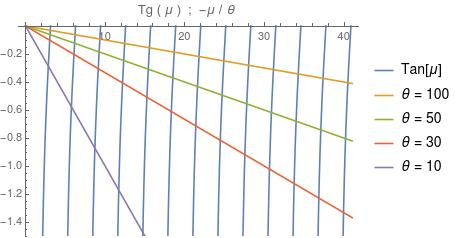
\includegraphics[scale=0.6]{Dibujo.jpg}
    \caption{En este ejemplo, se puede ver que la intersección entre $Tan(x)$ y $-x$ tiende a las asíntotas verticales de la tangente, el mismo comportamiento se aprecia para cualquier $ \theta $.}
    \label{fig:Dibujo1}
\end{figure}

\begin{equation}
\begin{array}{c}
    \mu _n = n \pi + \frac{\pi}{2} + \epsilon _n \\
    Donde \ \epsilon _n \rightarrow{0}  \ cuando \ n \rightarrow{0}
\end{array}
\label{eq.mu}
\end{equation}


Conocer $\epsilon _n $ es equivalente a resolver la ecuación (\ref{eq.asintota}) la cual no posee solución analítica, en vez de eso voy a obtener un desarrollo de $\epsilon _n $ para $n \rightarrow \infty$.

Voy a insertar (\ref{eq.mu}) en la segunda ecuación de (\ref{eq.asintota}) y desarrollar alrededor de $\epsilon \rightarrow{0}$ obteniendo:

\begin{equation}
\begin{array}{c}
    Sin( n \pi + \frac{\pi}{2} + \epsilon _n ) = 
    - \frac{n \pi + \frac{\pi}{2} + \epsilon _n}{\theta}  \ Cos( n \pi + \frac{\pi}{2} + \epsilon _n )  \\
 \\

         (-1) ^n \sum _{p=0} ^{\infty} \frac{(-1) ^p  \epsilon _n ^{2 p }}{(2p)!} 
    =  \frac{-(n \pi + \frac{\pi}{2} + \epsilon _n) }{\theta}  \  \	
    (-1) ^n
     \sum _{p=0} ^{\infty} \frac{(-1) ^ {p+1} \epsilon _n ^{2 p + 1}}{(2p+1)!} 
\end{array}
\end{equation}


Donde acomodando la igualdad, obtengo la ecuación :

\begin{equation}
    1 = 
    \sum _{p=0} ^{\infty} (-1) ^p     \left[
   	\epsilon _n ^{2p+2 }\left( \frac{1}{(2p+1)! \theta } + \frac{1}{(2p+2)} \right) +
  	\frac{n \pi + \frac{\pi}{2}}{\theta} \frac{  \epsilon _n ^{2p+1}}{(2p+1)!} 			\right]
\label{igualdad epsilon}
\end{equation}

Suponiendo que $\epsilon _n $ tiene un desarrollo en serie de la forma .

\begin{equation}
    \epsilon _n = 
    \frac{\epsilon ^{(1)}}{n}  + 
    \frac{\epsilon ^{(2)}}{n ^2}  + 
    \frac{\epsilon ^{(3)}}{n ^3}  + ...
\label{eq.epsilon}
\end{equation}


Insertando el desarrollo de $\epsilon$ en la ecuación (\ref{igualdad epsilon}), e igualando orden a orden se obtiene:

\begin{equation}
    \epsilon _n = \frac{\theta}{n \pi} 
     - \frac{ \theta}{2 \pi n ^2 } + O \left( \frac{1}{n ^3}\right)
\label{epsilons}
\end{equation}

Una vez obtenido el desarrollo de $\mu _n $ puedo calcular $\lambda _n = \frac{\mu _n }{L}  $ 



\begin{equation}
    \lambda _n = 
	\frac{n \pi}{L} + 
    \frac{\pi}{2 L} +
    \frac{\gamma}{n \pi} -
    \frac{\gamma}{2 n ^2 \pi} +
    O \left(  \frac{1}{n^3} \right) 
\end{equation}
    
Voy a obtener para la función $ \zeta _A (s)$ a este orden:
    
\begin{equation}
\begin{array}{cc}
    \zeta _{A} (s) =  
    \sum _{n=1} ^{\infty} 
    \left( \frac{\lambda _n }{\mu} 
    	\right) ^ {-2 s}  =
    \sum _{n=1} ^{\infty} 
    \left(
	\frac{n \pi}{L \mu} + 
    \frac{\pi}{2 L \mu} +
    \frac{\gamma}{n \pi \mu } -
    \frac{\gamma}{2 n ^2 \pi \mu } +
    O \left(  \frac{1}{n^3} \right) 
    \right) ^{-2 s} = \\
    ( \frac{L \mu }{\pi} ) ^{2s}    
    \sum _{n=1} ^{\infty} 
    n ^{- 2 s} 
    \left(
    1 +     
    \underbrace{
        \frac{1}{2 n} + 
        \frac{L \gamma}{n^2 \pi ^2} -
        \frac{L \gamma}{2 n ^3 \pi ^2} +
        O(\frac{1}{n ^{4}} ) } _{ \chi _n}
    \right ) ^{-2 s}
\end{array}
\end{equation}

Para calcular esta serie voy a hacer un desarrollo binomial alrededor de $\chi _n \rightarrow{0} $  .

\begin{equation}
\begin{array}{c}
\zeta _{A} (s) = 
( \frac{L \mu }{\pi} ) ^{2s}
\sum _{n=1} ^{\infty}
  n  ^{-2 S} \\
(
	1 - 
	2 s \chi _n +  s(2s+1) \frac{\chi _n ^2}{2} - 
	\frac{2}{3} s(2s+1)(s+1) \chi _n ^3  + O( \frac{1}{n ^4}) )

\end{array}
\end{equation}

Se desarrolla hasta este orden, porque hay que tener en cuenta que cada termino $\chi _{n} ^{m} $ contribuye al orden mas bajo en la sumatoria en una potencia $\frac{1}{n ^m}$, el resultado final es:





\begin{equation}
\begin{array}{c}
    \zeta _A (s) = \left( \frac{L \mu }{\pi} \right) ^{2s} \\
	\Bigg(
		\zeta ( 2 s ) -
		s \zeta ( 2s+1 ) +
		 \zeta (2s +2 ) s \left( \frac{1}{4} + \frac{s}{2} - \frac{2 L  \gamma}{\pi ^2} \right)  \\
		 - \zeta (2s+3) \left(  
							\frac{s(s+1) ( \pi ^2 + 2 \pi ^2 s - 24 L \gamma)}{12 \pi ^2 }
		 					\right) 
		+ ...
		\Bigg)
\end{array}
\end{equation}


Los polos de mi función $\zeta _A (s)$ estarán dados por los polos de las funciones $\zeta (s+n)$, desarrollando en los primeros polos obtengo:

\begin{equation}
\begin{array}{c}
\zeta _A (s \rightarrow 1/2) = 
\frac{L \mu }{2 \pi } \frac{1}{s-1/2} + \ finito \\
\zeta _A (s \rightarrow 0) = \ finito \\
\zeta _A (s \rightarrow -1/2) = \frac{\gamma}{2 \pi \mu } \frac{1}{s+1/2} \\
\zeta _A (s \rightarrow -1) = finito \\
\end{array}
\end{equation}

Lo cual corrobora que los polos están en semienteros de $s$.

\subsection{Calculo de la función zeta mediante calculo complejo:}

Conocida la ecuación de autovalores, se puede proceder a calcular la función $\zeta _A (s) $ sin calcular explícitamente los autovalores.

Si los  autovalores están definidos por una función $f(\lambda ) = 0$, de la cual son ceros simples, entonces la función $f'(z) / f(z) $ va a tener polos simples en los autovalores de $\hat{A}$, así la  función $\zeta _A (s)$ va a poder representarse como una integral en el plano complejo, donde el camino de intregración es cualquiera de los dos caminos representados en la figura [\ref{autovalores}]:

\begin{equation}
\begin{array}{c}
   \zeta _A (s) =  \sum _{n=1} ^{\infty} \left( \frac{\lambda _n}{\mu} \right) ^{-2s} = \\ 
   \frac{1}{2 \pi i} \int _{C} \frac{f'(z)}{f(z)} \left( \frac{z}{\mu} \right) ^{-2s} dz =  
    \frac{1}{2 \pi i} \int _{C}
    \frac{ cos(L z) \left(L + \frac{1}{\gamma} \right) - sin(L z) \frac{z L}{\gamma}
    }
    {cos(L z) \frac{z}{\gamma} + sin(L z)
    }
    \left( \frac{z}{\mu} \right) ^{-2 s} dz
\end{array}
\end{equation}


\begin{figure}
\centering
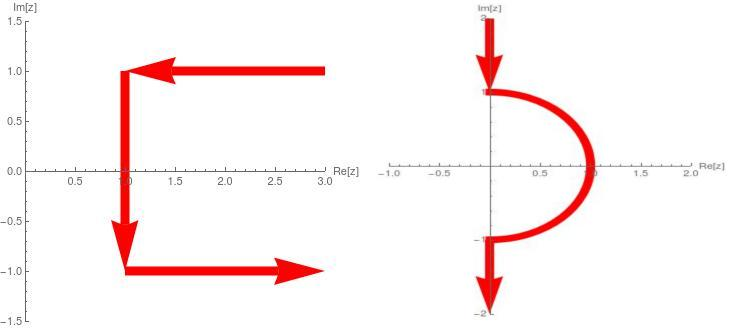
\includegraphics[scale=0.3]{contorno.jpg}
\caption{Camino tenido en cuenta para realizar la integral de contorno en el plano complejo}
\label{fig:contorno}
\end{figure}


Voy a utilizar el camino de la derecha de [\ref{fig:contorno}], el cual puedo descomponer en 3 integrales, una angular y dos rectas, la contribución angular es regular para todo s, entonces no aporta a la estructura de polos, en cuanto a las contribuciones del lado recto voy a realizar mi integral en función de t, parametrizando z de la forma $z = \pm i  t$, luego de tirar los términos exponencialmente decrecientes obtengo:

\begin{equation}
    \frac{Sin(\pi s)}{ \pi } 
    \int _1 ^{\infty} 
    t ^{-2s}
    \underbrace
    {
	\frac{ \frac{1}{\gamma} + L + \frac{L t}{\gamma}}
	{1+ \frac{t}{\gamma}}
	} _{\chi}
    dt 
\label{contorno}
\end{equation}

En donde voy a insertar el desarrollo asintótico de   $\chi$. 

\begin{equation}
    \chi = L +  \sum _{n=1} ^{\infty} \frac{(-1) ^{n+1} \gamma ^{n-1} }{t ^n}
\label{eq:chi}
\end{equation}

Luego de integrar termino a termino, obtengo como resultado:

\begin{equation}
    \zeta _A (s) = 
    \frac{Sin(\pi s)}{\pi} 
    \left(
    \frac{L}{2s-1} + 
    \sum _{n=1} ^{\infty}
    \frac{(-1) ^{n+1} \gamma ^{n-1} }{2s+n-1}
    \right)
\label{eq.zeta.com}
\end{equation}

De acá se puede ver que tiene polos simples en $s=1/2$ donde la estructura de polos queda determinada por

\begin{equation}
\begin{array}{c}

\zeta(s \rightarrow 1/2) = \frac{L}{2 \pi} \frac{1}{s-1/2} \\
\zeta (s \rightarrow -n - 1/2)  = \frac{ (-1) ^n \gamma ^{2n+1}  }{2 \pi} \frac{1}{s + n + 1/2}

\end{array}
\end{equation}


Que coincide con los polos calculados anteriormente.


\subsection{Uso del Heat-Kernel:}

En el capitulo anterior, se dio una expresión para el desarrollo del Heat-Kernel en el limite $t \rightarrow 0$, lo cual a través de la transformada de Mellin permite, conocer los polos de la función $\zeta _A (s)$, dada las condiciones de nuestro operador (variedad unidimensional, sin curvatura, sin potencial), los coeficientes del Heat-Kernel se van a simplificar considerablemente, quedando

\begin{equation}
\begin{array}{c}
C _0 (A) = \frac{1}{\sqrt{4 \pi}} \int _{0} ^{L} dx = \frac{L}{\sqrt{4 \pi}} \\
C _1 (A) = \frac{1}{4} \left( (-1) + (+1) \right) = 0 \\
C _2 (A) = \frac{12}{6} \frac{1}{\sqrt{4 \pi }} \left(  - \gamma \right) = - \frac{\gamma}{\sqrt{\pi}} \\
C _3 (A) = \frac{192}{384}  (- \gamma ) ^2 = \frac{\gamma ^2}{2} \\
C _4 (A) = \frac{480}{360} \frac{1}{\sqrt{4 \pi}} (- \gamma) ^3 = \frac{-2 \gamma}{3 \sqrt{\pi}}

\end{array}
\end{equation}

Insertando estos coeficientes en (REF) obtengo:

\begin{equation}
\begin{array}{c}
Res[ \zeta _A (s)] | _{s=1/2} = \frac{L}{2 \pi} \\
Res[ \zeta _A (s)] | _{s=0} = 0 \\
Res[ \zeta _A (s)] | _{s=-1/2} = \frac{\gamma}{2 \pi} \\
Res[ \zeta _A (s)] | _{s=-1} = \frac{\gamma}{2 \pi} = 0 \\
Res[ \zeta _A (s)] | _{s=-3/2} = - \frac{\gamma ^2}{2 \pi} = 0 \\


\end{array}
\end{equation}

Lo cual coincide con lo calculado por los dos métodos anteriores.


\chapter{Estudio del Problema Singular}

En este capitulo se van a aplicar las herramientas desarrolladas en el capitulo anterior al estudio del espectro de un operador singular

\section{El Operador Singular}

Como trabajo de tesis se propondra aplicar los metodos desarrollados en el capitulo anterior al operador diferencial (\ref{operador}).

\begin{equation}
\begin{array}{c}
    A \phi (x) = - \partial ^2 _x  \phi(x) + \frac{\alpha}{x} \phi(x) \\
    \phi(0) = \phi(L) = 0 
\end{array}
\label{operador}
\end{equation}

Para eso voy a resolver la ecuación de autovalores (\ref{eq.aut.sin}).

\begin{equation}
\begin{array}{c}
    A  \phi (x)  =   \omega ^2 \phi (x) \\ 
    \omega \ \in \ \mathfrak{R}
\end{array}
\label{eq.aut.sin}
\end{equation}

La cual posee soluciones LI $ y_1 $ y $ y_2 $ dadas por :

\begin{equation}
    \phi (x) = 
    \underbrace{
    C[1] \ e ^{-i \omega x} \ x \ F _{1} ^{1} (1+\frac{ \alpha}{2 \omega i },2,2 i \omega x) } _ {y_1}
    + \underbrace{C[2] \ e^{-i \omega x } \ x \ U (1+\frac{ \alpha}{2 \omega i },2,2 i \omega x) } _{y_2} 
\end{equation}


%Para autovalor $- \omega ^2 $ obtengo las siguientes soluciones:

%\begin{equation}
%    \phi ^{-} (x) = 
%    \underbrace{
%    C[1] \ e ^{-i \omega x} \ x \ F _{1} ^{1} (1 + \frac{ \alpha}{2 \omega},2,2 i \omega x) } _ {y_1}
%    + \underbrace{C[2] \ e^{-i \omega x } \ x \ U (1 + \frac{ \alpha}{2 \omega},2,2 i \omega x) } _{y_2} 
%\end{equation}

Donde $F _1 ^1(a,b,z)$ y $ U(a,b,z)$ son las soluciones LI de la ecuacion hypergeometrica (\ref{eq:hyper})

\begin{equation}
    z \ \partial ^2 _z \ \psi (a,b,z) + (b-z) \
    \partial _z \psi (a,b,z)
    -a \ \psi (a,b,z) = 0
\label{eq:hyper}
\end{equation}

Las cuales tienen las siguientes expresiones analiticas  : 

\begin{equation}
\begin{array}{c}
	U(a,b,z) = \frac{1}{\Gamma (a)} 
	\int _0 ^{\infty} e ^{-zt}
	t ^{a-1}
	(1+t) ^{b-a-1}
	dt \\
	F _1 ^1 (a,b,z) = \sum _ {k=0} ^{\infty} 
	\frac{(a) _k}{(b) _k} 
	\frac{z ^k}{k!} 
\end{array}
\end{equation}

%\textbf{Estados Ligados:} \\

%Primero voy a buscar estados ligados, imponiendo la condicion $\phi ^{-} (0) = 0$, veo que $U(1- \frac{\alpha}{2 \lambda} ,2 ,0) \rightarrow \infty $ obtengo $C[2] = 0$

%Los estados ligados van a surgir entonces de la condicion de contorno en $x=L$

%\begin{equation}
%	F _1 ^{1} (1- \frac{\alpha}{2 \omega} , 2 2 i \omega L ) = L 
%\end{equation}


\textbf{Estados de Scattering:} \\
%    A partir de aquí $\phi ^{+} (x)$ la escribiré $\phi (x)$ \\


Para aplicar la condicion de contorno $\phi (0) = 0$, hay que hacer un desarrollo de $\phi(x \rightarrow 0)$, el cual es:

\begin{equation}
\begin{array}{c}
\phi (x \rightarrow 0) \approx
C[1] ( x + O(x ^2)) + 
C[2] x 
\left( 
\frac{1}{  \alpha x  \Gamma ( \frac{ \alpha}{2 i \omega}  )   }  +
\frac{Log[x] }{\Gamma ( \frac{ \alpha}{2 i \omega} ) } + Cte + O(x)
\right)
\\
Donde,  \ Cte = 
\frac{
-1 + 2 \gamma + Log[2 i \lambda] + \psi (1 + \frac{ \alpha}{2 i \omega})
}
{\Gamma (\frac{i \alpha}{2 \lambda})}
\end{array}
\label{eq.scat}
\end{equation}

Donde se ve que $y _1 (x \rightarrow 0 ) \rightarrow 0$ y $y _2 (x \rightarrow 0)  \rightarrow
\frac{1}{  \alpha   \Gamma ( \frac{i \alpha}{2 \lambda}  )   } $ , entonces la forma de satisfacer la condicion de contorno es poniendo C[2] = 0

Los autovalores estaran dados entonces por los ceroes de $y_1 (x= L)$, como el único termino que se anula en el produco es la funcion Hypergeometrica, los autovalores vienen dados por los ceros de la ecuacion (\ref{eq.1}), donde se puede ver su comportamiento en la figura (\ref{fig:funcion}) en funcion de $\omega$ para  $\alpha=1, \ L=1$.:


\begin{equation}
y_1 (L, \omega) = F _1 ^1 (1+\frac{ \alpha}{2 i \omega},2,2 i \omega L)  = 0
\label{eq.1}
\end{equation}

\begin{figure}
\centering
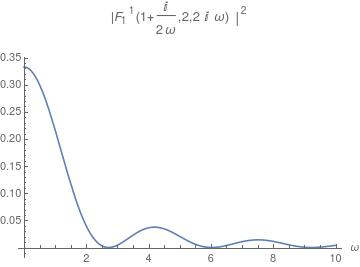
\includegraphics[scale=0.7]{Funcion.jpg}
\caption{En esta imagen se puede ver el comportamiento de los ceros de función $F _1 ^1$, para $\alpha=1$ y $L=1$}
\label{fig:funcion}
\end{figure}

A partir de ahora en vez de trabajar con la función $F _1 ^1$, voy a trabajar con el primer termino de su desarrollo en serie a $ \omega \rightarrow \infty  $ dado por (\ref{eq.aprox}) 

\begin{equation}
    F _1 ^1 (a,b,z) = \Gamma (b) 
    \left(
    \frac{e^z z ^{a-b} }{\Gamma(a)} * A_1 + \frac{(-z) ^{ -a}}{ \Gamma(b-a)} 
    * A_2
    \right)
\label{eq.aprox}
\end{equation}

Donde $A_1$ y $A_2$ son los demas terminos de la serie, que voy a tomar como 1, en el apéndice 1 voy a demostrar que no contribuyen a la estructura de los polos al orden que estoy calculando, si hay que tenerlos en cuenta para calcular los polos mas halla de donde se calcularon en esta tesis.

Definiendo las variables adimensionales $\mu = \omega L$  y $\beta = \alpha L $ y reemplazando los valores correspondientes en la ecuación (\ref{eq.aprox}) obtengo. 

\begin{equation}
    F _1 ^1 (1+  \frac{  \beta}{2 i \mu} ,2 ,2 i \beta ) = 
   i  \frac{e ^{- \frac{\pi}{4} \frac{\beta}{\mu} } }{2 \mu}
    \left( -
    \frac{e ^{- i \frac{\beta}{2 \mu} Ln(2 \mu) } e ^{2 i \mu} }{\Gamma(1+\frac{ \beta}{2 i \mu})} +
    \frac{e ^{  i \frac{\beta}{2 \mu} Ln(2 \mu) }}               {\Gamma(1-\frac{ \beta}{2 i \mu})}
    \right)
\label{eq.completa}
\end{equation}




La cual queda expresada como un producto de dos funciones, una parte que se anula y una parte que no.

Para obtener los autovalores voy a solo ocuparme de la parte que se anula, la cual esta entre paréntesis.

\begin{equation}
    M (\mu) = -
    \frac{e ^{- i \frac{\beta}{2 \mu} Ln(2 \mu) } e ^{2 i \mu} }{\Gamma(1+\frac{ \beta}{2 i \mu})} +
    \frac{e ^{  i \frac{\beta}{2 \mu} Ln(2 \mu) }}               {\Gamma(1-\frac{ \beta}{2 i \mu})}
\label{eq.aproxx}
\end{equation}

Para el calculo de la funcion $\zeta _A (s) $ se puede utilizar ($\mu$) o cualquier multiplo de ella, ya que posee los mismos autovalores que $F_1 ^1 $

%En todas las cuentas posteriores, para calcular $\zeta _A (s)$ voy a utilizar $M ( \mu )$ ya que posee los mismos autovalores de $ F _1 ^1 $.



\section{Calculo Asintótico de los autovalores}



Necesito conocer los ceros de  de $M(\mu)$ a $\mu \rightarrow{\infty}$, suponiendo que $\mu _n$ la puedo descomponer en una parte divergente mas una infinitesimal cuando $n \rightarrow{\infty}$, tal como en el capitulo anterior.

Para que el desarrollo sea mas simple, voy a voy a escribir a $M (\mu)$ como :

\begin{equation}
M (\mu) = e ^{\frac{i \beta Log[2 \mu]}{\mu}}
\frac{\Gamma (1- \frac{i \beta}{2 \mu})}{\Gamma (1 + \frac{i \beta}{2 \mu})}
- e ^{2 i \mu}
\label{eq.otro.mu}
\end{equation}


En el limite de $\mu _n \rightarrow \infty$ se obtiene:

\begin{equation}
    M(\mu _n \rightarrow \infty) = 
	1 - e ^{2 i \mu}
\end{equation}

De acá se puede ver que el comportamiento de $\mu _n$ esta dado por 


\begin{equation}
\begin{array}{c}
    \mu _n = n \pi + \epsilon _n \\
    Donde \ \epsilon _n \rightarrow{0} ,\ si \ n \rightarrow{0}
\end{array}
\label{eq.mu2}
\end{equation}



Para calcular orden a orden el termino $\epsilon _n$ inserto la ecuación (\ref{eq.mu2}) en (\ref{eq.otro.mu}) e igualo la ecuación a cero, lo cual conduce a la siguiente ecuación para $\mu _n$

\begin{equation}
	e ^{ i \frac{\beta}{ \mu _n} Ln(2 \mu _n)}     
    \frac{\Gamma(1 + \frac{ \beta}{2 i \mu _n} ) }
    {\Gamma(1 - \frac{ \beta}{2 i \mu _n})} =    
    e ^{2 i \epsilon _n }
\end{equation}

teniendo en cuenta que $\frac{ln(2 \mu _n)}{2 \mu _n }$ tiende a cero a $\mu _n$ grade, puedo hacer un desarrollo de la exponencial y las funciones $\Gamma$ alrededor de $ \mu \rightarrow \infty $, y $\epsilon \rightarrow 0$

\begin{equation}
    \left(
    \sum _{p = 0} ^{\infty} \frac{( i \frac{\beta}{ \mu} Log[2 \mu]) ^p }{p!}
    \right)
    \left(
	\sum _{q = 0} ^{\infty} \frac{a _q}{\mu ^q}
	\right)
    =
    \left(
    \sum _{l = 0} ^{\infty} \frac{( 2 i \epsilon)^l}{l !}
    \right)
\end{equation}


Al orden mas bajo se obtiene la ecuación : 

\begin{equation}
(1 + \frac{i \beta}{ \mu} Log[2 \mu)] 
(1 + \frac{i  \gamma \beta}{ \mu})  =
(1 + 2 i \epsilon)
\end{equation}

Todo esto conduce a que el termino subdominante sea $\epsilon _n =  \frac{\beta Ln(2 n \pi)}{2 n \pi}$ , pero con esto no alcanza, ya que existe un termino que decae como 1/n, entonces para calcular el polo que nos interesa se deben calcular todos los términos que decaigan como 1/n, insertando $\epsilon _n =  \frac{\beta Ln(2 n \pi)}{2 n \pi} + \epsilon '$ en la ecuación anterior, obtengo:


\begin{equation}
    \epsilon _n =  \frac{\beta Ln(2 n \pi)}{2 n \pi} 
                \frac{\gamma \beta}{2 n \pi} +
                O(\frac{1}{n^2})
\end{equation}

Luego para calcular la función $\zeta _{A}$ utilizo su definición

\begin{equation}
\begin{array}{c}
    \zeta _A (s) = \sum _n ^{\infty} \omega _n ^{-s}  =
    \sum _{n=1} ^{\infty} \left(\frac{\mu _n}{L} \right) ^{-2 s} =  \\
    L ^{2 s} \sum _{n=1} ^{\infty} 
    \left( 
    n \pi + \frac{\beta Ln(2 n \pi)}{2 n \pi} + \frac{\gamma \beta}{2 n \pi} +
    O(\frac{1}{n^2})
    \right) ^{-2s} = \\
    
\end{array}
\end{equation}

Como en el ejemplo anterior puedo escribir todo como

\begin{equation}
\begin{array}{c}
    \zeta _A (2 s) = \left( \frac{L}{\pi} \right)  ^{2 s} 
    \sum _{n=1} ^{\infty} n ^{- 2  s}
    \left(
    1 - \frac{\beta Ln(2 n \pi)}{2 n^2 \pi ^2} - \frac{\gamma \beta}{2 n^2 \pi ^2 } +
    O(\frac{1}{n^3})  \right) ^{-2 s} = \\
    \sum _{n=1} ^{\infty} n ^{-2 s} 
    \left(
    1 -\chi _n \right) ^{- 2 s}
\end{array}
\end{equation}

Utilizando como en el ejemplo anterior el desarrollo de la ecuacion para $\chi \xrightarrow 0$, puedo expresar mi funcion zeta como 


\begin{equation}
\begin{array}{c}
    \zeta _A (s) = ( \frac{L}{\pi} ) ^{2 s}
    \sum _{n=1} ^{\infty} 
    n ^{-2s}
    \left(
    1 + 2 s \chi + O(\chi ^2)
    \right) =  \\
    ( \frac{L}{\pi} ) ^{2 s}
    \left(
    \sum _{n=1} ^{\infty} n ^{-2 s} 
    \left(
    1 - 2s (
    \frac{\beta Log[2 n \pi]}{2 n ^2 \pi ^2} + 
    \frac{\gamma \beta}{2 n ^2 \pi ^2} +
    O (n ^{-3}  )
    \right)
    \right)
\end{array}
\end{equation}


\begin{equation}
\begin{array}{c}
    \zeta _A (S) = 
    \left( \frac{L }{ \pi } \right) ^{2}  \\
    \left(
    \zeta (2 S) -
	\frac{ s \beta}{ \pi ^2}
	\left(
	\zeta (2s+2)  ( Log[2 n \pi ] + \gamma) +
	\zeta '(2s+2) \
	\right)
    \right)
\end{array}
\end{equation}

Donde sabiendo que $\zeta(s) = \frac{1}{s-1} + Regular$, el primer polo queda determinado como

\begin{equation}
    Res(s=1/2) = \frac{L}{2 \pi}    
\end{equation}

Aquí sabiendo el desarrollo de $\zeta(s)$ alrededor de $s=1$ puedo conocer los desarrollos de $\zeta'(2s+2)$, que lo utilizo para desarrollar alrededor de mi segundo polo en $s = -1/2$ obteniendo:

\begin{equation}
    \zeta _A (s) =  \frac{\beta}{8 L \pi (s+1/2)^2} +
    \beta \frac{(-1 + \gamma + Log[2L ])}{4 L \pi (s+1/2)} + 
    Regular
\end{equation}

\section{Calculo Utilizando Variable Compleja}


Sabiendo que los autovalores de mi Hamiltoniano son todos reales, puedo expresar $\zeta _A (s)$ como una integral en el plano complejo, y deformar la trayectoria hasta el camino dado por la figura [\ref{fig:contorno}], tal como se hizo en el capitulo anterior: \\

Mi funcion $ \zeta _A (s) $ va a quedar definida por:

\begin{equation}
\zeta _A (s) = 
\frac{1}{2 \pi i} 
\int _{\mathcal{C}}
\frac{M ' ( \mu ) }{ M ( \mu ) } d \mu
\label{eq.zeta.compleja}
\end{equation}

Donde $M ( \mu )$ está dada por (\ref{eq.aproxx}).
cuando integre los ejes verticales, voy a obtener un termino exponencialmente decreciente y uno decreciente, que se van a alternar dependiendo de si estoy arriba o abajo del eje real. \\

Reemplazando la parametrizacion $ \mu  (t) = \pm i t$ en (\ref{eq.zeta.compleja}) y tirando los terminos exponencialmente decrecientes, obtengo:


\begin{equation}
\begin{array}{c}
    \zeta _A (s) = \\
     \frac{1}{2 \pi i} \int _{\infty} ^{1}
     \frac{\beta}{2 t^2} 
     \left(
     1 - \frac{i \pi}{2} + Log[2 t] + \psi (1 + \frac{\beta}{2 t})
     \right)
     t ^{-2s}
     e ^{- i \pi s} (i dt) + \\
     \frac{1}{2 \pi i} \int _{\infty} ^{1} 
     \left(
     2 + \frac{\beta}{2 t^2}
     \left(
     1 + \frac{i \pi}{2} - Log[2 t] - \psi (1+ \frac{\beta}{2 t})
     \right)
     t ^{-2s}
     e ^{ i \pi s} (-i dt)
     \right)     
\end{array}
\end{equation}

\begin{equation}
\begin{array}{c}
    \zeta _A (s) = \\
     \frac{1}{2 \pi i} \int _{\infty} ^{1}
     \frac{i \alpha}{2 t^2}
     \left(
     1 - Log(2 L t) - \frac{i \pi}{2} + \psi (1-\frac{\alpha}{2 t})
     \right)
     t^{-2 s}
     e^{-i \pi s} \ 
     (i dt) + \\
     \frac{1}{2 \pi i} \int _1 ^{\infty}
     \frac{ \alpha}{2 i t^2}
     \left(
     \left(
     1 - Log(2 L t) - \frac{i \pi}{2} + \psi (1-\frac{\alpha}{2 t}) 
     \right)
     + 2 i L
     \right)
     t^{-2 s}
     e^{i \pi s}
     (-i dt)
     
\end{array}
\end{equation}

Donde antes de reacomodar los terminos puedo calcular el termino que contiene $2iL$ el cual es la potencia mas alta de $t$ para obtener: 

\begin{equation}
    \frac{1}{2 \pi i }
    \int _1 ^{\infty}
    2 i L
    e^{i \pi s}
    t ^{-2 s}
    (-i dt) =  
    \frac{L e^{i \pi s} }{2 \pi i} \frac{1}{s-1/2   }
\end{equation}

Ningún otro termino aportará a este polo, entonces el residuo en $s= 1/2$ es:

\begin{equation}
    Res (s=1/2) = \frac{L}{2 \pi}
\end{equation}

Que se corresponde con el calculado con el método anterior. \\

Una vez calculado este termino, puedo reorganizar el resto de la integral como:

\begin{equation}
\begin{array}{c}
    - \frac{\alpha}{2 \pi} \ sin[\pi s]
    \int _1 ^{\infty}
    t ^{-2 s-s} 
    \left(
    1 - Log[2Lt] + \psi (1- \frac{\alpha}{2t})
    \right) dt - 
    \frac{\alpha}{4} 
    Cos[\pi s]
    \int _1 ^{\infty} t^{-2s-s} dt
\end{array}
\end{equation}

Donde todos los términos son calculables analíticamente, excepto el que esta multiplicado por $\psi$, para lo cual utilizo el desarrollo de $\psi$ en $t \rightarrow \infty$:

\begin{equation}
    \psi(1-\frac{\alpha}{2 t}) \approx 
    -\gamma + O(\frac{1}{t})
\end{equation}

Realizando todas las integrales la funcion $ \zeta _A (s)$ a este orden queda determinada por:  

\begin{equation}
\begin{array}{c}
    \zeta (s) _{A} = 
    \frac{L e ^{i \pi s}}{2 \pi i} \frac{1}{s-1/2} 
    -\frac{\alpha Sin[\pi s]}{4 \pi} \frac{1}{s+1/2} \\
    \alpha 
    \frac{
    1+S Log(4)+2SLog[L]+Log[2L]
    }
    {8 \pi} \frac{sin(\pi s)}{(s+1/2) ^2}  \\
    \frac{\gamma \alpha Sin[\pi s]}{4 \pi } \frac{1}{s+1/2} 
    \frac{\alpha cos(\pi s) }{8 \pi}  \frac{1}{s+1/2}  \\
\end{array}
\end{equation}

Donde el siguiente termino en el desarrollo de $ \psi $ contribuirá al residuo en $s = -3/2$

Para calcular el residuo en $s=-1/2$ desarrollo todo en Serie de Laurent alrededor de ese punto obteniendo.

\begin{equation}
    - \frac{\alpha}{8 \pi} \frac{1}{(s+1/2)^2} + 
    \alpha \frac{1-\gamma -Log[2 L]}{4 \pi} \frac{1}{s+1/2} + \ Regular
\label{eq.desarrollo}
\end{equation}

Donde se puede ver que el residuo, y la contribución al polo cuadrático en $s=-1/2$ coinciden con las calculadas anteriormente.

%Una aclaracion importante es que el termino $Log[2 L ]$ es correcto dimensionalmente, ya que proviene de evaluar la integral $\int _1 ^\infty  Log[2 L \omega] \ d \omega$

\section{Cálculo de la energía de vacío}

La energía de vacío queda determinada por la ecuación 

\begin{equation}
    E _0 = \frac{\hbar}{2}  
    \zeta (s)  |  _{- \frac{1}{2}}
\end{equation}

$\zeta (s)$ ya está desarrollada alrededor de $s=-1/2$ en (\ref{eq.desarrollo}), queda desarrollar $(E_c) ^{2s+1} $ alrededor de $s=-1/2$ quedando.

\begin{equation}
    E _c \approx 
    1 + 2 Log[E_c] (s + 1/2) +
    2 Log[E_c] ^2 (s+1/2) ^2 + 
    O (s+1/2)^3
\end{equation}

Entonces la energía de vació queda determinada por:

\begin{equation}
    E _0 =
    \left(
    \frac{1}{(s+1/2)^2} 
    \left(
    \frac{- \alpha}{8 \pi}
    \right)+
    \frac{
    \alpha(1 -\gamma-Log[2L]) - 
    \alpha Log[E_c] 
    }{4 \pi (s+1/2)} 
     + Regular
    \right) | _{s=-1/2}
\end{equation}


\chapter{Limite Continuo}

En esta seccion voy a estudiar el comportamiento de la fucion $\zeta (s) $ en el limite $L \rightarrow \infty$, donde quedara definida por:

\begin{equation}
\zeta (s) = \int _{0} ^{\infty} \rho (x) x^{-2 s} dx
\end{equation}

Donde la $\rho(x) $ es la densidad de autovalores, para llegar a esta ecuacion, voy a utilizar la representacion integral de la funcion $\zeta$ en el plano complejo e integrar sobre un camino dado por la figura(REFERENCIAR), para eso voy a trabajar con mi aproximacion (REFERENCIAR)



Dependiendo si estoy arriba o abajo del eje real, voy a tener un termino exponencialmente creciente/decreciente en el limite $L \rightarrow \infty$ proveniente de $e ^{i z t}$

Voy a separar mi integral en una parte de arriba y una parte de abajo, en el termino de arriba del eje real obtengo:

\begin{equation}
\begin{array}{c}
\frac{1}{2 \pi i} \int _{\infty} ^{t0} 
\partial _z
Log
\left(
\frac{e ^{-2 i z  L } e ^{- \frac{i \alpha}{2 \lambda} Log[2 z  L]} }{\Gamma[1-\frac{i \alpha}{2 z }]} +
\frac{e ^{ \frac{i \alpha}{2 z } Log[2 z  L]} }{\Gamma[1+\frac{i \alpha}{2 z }]}
\right) d z \\
z = i t + \epsilon 
\end{array}
\end{equation}

Sacando factor comun de modo que me quede un termino exponencialmente decrenciente dentro del Logatirmo obtengo

\begin{equation}
\frac{1}{2 \pi i}  \int _{\infty} ^{t0} 
\partial _{z}
\left(
\frac{i\alpha}{2 z} Log[2 z L] - Log[\Gamma[1 + \frac{i \alpha}{2 z}]] +
Log[1- \epsilon _L ]
\right)
d z
\end{equation}

Donde $ \epsilon _L \rightarrow 0$ si $L \rightarrow \infty $ , entonces Logaritmo va a cero, quedando la integral final:

\begin{equation}
\begin{array}{c}
\zeta (s) = 
\frac{L}{\pi}
\int _ {x_0} ^{\infty} x ^{-2s} dx + \\
\frac{\alpha}{2 \pi } \int _{x_0} ^{\infty} 
\left(
\frac{-1}{ x ^2} -
\frac{Log[2 x L]}{x ^2}  -
\frac{1}{ x ^2 } 
\left(
\psi (1 + \frac{i \alpha}{2 x}) + \psi (1 - \frac{i \alpha}{2 x}) 
\right)
\right)
x ^{-2s} d x
\end{array}
\end{equation}



Relizando las integrales termino a termino obtengo

\begin{equation}
\begin{array}{c}
\zeta (s) = 
\frac{\alpha}{2 \pi} x _{0} ^{-2s-1}
\left( 
\frac{1}{(1+2s) ^2} +
\frac{Log[2 L x _0]}{1+2s} -
\frac{1}{1+2s}
\right) + 
\frac{L}{\pi} \frac{x _0 ^{-2s+1}}{2s-1}  \\
- \frac{\alpha}{2 \pi}
\int _{x_0} ^{\infty} 
\left(
\psi(1 + \frac{i \alpha}{2 x}) +
\psi(1 - \frac{i \alpha}{2 x} )
\right)
x ^{-2s-2}
dx
\end{array}
\end{equation}


Para calcular el ultimo termino hay distintos desarrollos en serie de la funcion $\psi $ que se pueden usar, yo voy a el desarrollo 

\begin{equation}
\begin{array}{cc}
\psi (1+ z ) = - \gamma + \sum _{n=2} ^{\infty} (-1) ^n \zeta (n) z ^{n-1} & |z| < 1
\end{array}
\end{equation}

El cual su radio de convergencia esta centrado alrededor de $x = 0$

La ultima integral queda expresada como:

\begin{equation}
\int _{x_0} ^{\infty}
\left(
-2 \gamma + 
2 \sum _{n=2} ^{\infty}
\zeta (2n+1) (-1) ^{n+1}
( \frac{\alpha}{2 x} ) ^{2n}
\right)
x ^{-2s-2} dx
\end{equation}

Quedando la funcion $\zeta _A (s) $ :

\begin{equation}
\begin{array}{c}
\zeta _A (s) = 
\frac{L x0 ^{-2s+1} }{2 \pi } \frac{1}{s- 1/2} + 
\frac{\alpha x0 ^{-2s-1} }{8 \pi } \frac{1}{(s+1/2) ^2} + \\
\frac{\alpha x0 ^{-2s-1} }{4 \pi } 
\left(
Log[2 L x_0] + \gamma - 1
\right)
\frac{1}{s+1/2} + \\
\frac{x_0 ^{-2s}}{2\pi} 
\sum _{n=1} ^{\infty} (-1) ^{n} \zeta (2n+1) 
( \frac{\alpha}{2 x0} ) ^{2n+1} \frac{1}{s+n+1/2}
\end{array}
\end{equation}

Para ver la energía de vacío hay que evaluar esta expresion en $s=-1/2$ y graficar su parte finita, tal como esta en la figura [ \ref{fig:vacio} ] donde estan los primeros 100 terminos de la serie, en funcion de $x = \alpha / x_0$ y la suma exacta de la serie al reemplazar $\zeta (2s+1) = 1$.

\begin{figure}
    \centering
    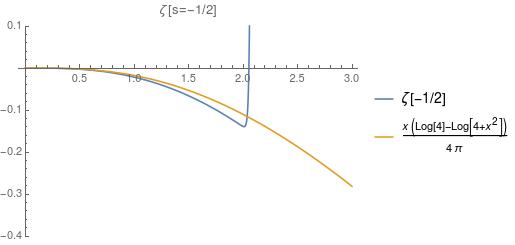
\includegraphics[scale=0.3]{Vacio.jpg}
    \caption{En esta imagen esta graficada la parte finita de la $\zeta _A (-1/2) $ en funcion del parametro $x= \frac{\alpha}{x _0}$ donde se sumaron los primeros 100 terminos de la serie, y en azul se puede ver la suma de la serie al reemplazar $\zeta (2n+1) = 1$}
    \label{fig:vacio}
\end{figure}
\chapter{Limite Continuo}

En esta sección se va a estudiar la función $\zeta (s) $ en el limite $L \rightarrow \infty$, donde la función $\zeta _A (s)$ va a quedar definida por:

\begin{equation}
\zeta (s) = \int _{0} ^{\infty} \rho (x) \ \left( \frac{x}{\mu } \right) ^{-2 s} dx
\end{equation}

Donde la $\rho(x) $ es la densidad de autovalores, para llegar a esta representación se utilizó la representación integral, donde el camino de integración de está dado por la figura izquierda de (\ref{fig:contorno}). La parametrización usada fue:


\[
z(t) =  
	  \begin{cases} 
      t + i \epsilon  & x _0 \leq t \leq \infty \\
      t - i \epsilon  & x _0 \leq t \leq \infty \\
      x _0 + i t		  & - \epsilon \leq t \leq \epsilon
   \end{cases}
\]

De (\ref{larga}) se puede ver que $S1,S2 \rightarrow 1$ cuando $L \rightarrow \infty$, por lo tanto se va a utilizar $M ( \lambda)$ dada por (\ref{eq.completa}).\\



Dependiendo si se está arriba o abajo del eje real, va a existir un termino exponencialmente creciente/decreciente en el limite $L \rightarrow \infty$ proveniente de $e ^{i z t}$

La integral correspondiente a arriba del eje real es:

\begin{equation}
\begin{array}{c}
\frac{ 1 }{2 \pi i} \int _{\infty} ^{t0} 
\partial _z
Log
\left(
\frac{e ^{-2 i z  L } e ^{- \frac{i \alpha}{2 \lambda} Log \left( 2 z  L \right) } }
	 {\Gamma \left( 1 + \frac{ \alpha}{2 i z } \right)} +
\frac{e ^{ \frac{i \alpha}{2 z } Log \left( 2 z  L \right)  } }{\Gamma \left( 1 - \frac{ \alpha}{2 i z } \right) }
\right) d z \\
z = i t + \epsilon 
\end{array}
\end{equation}

Sacando factor común de modo de obtener un termino exponencialmente decreciente adentro del logaritmo se obtiene:

\begin{equation}
\frac{ 1 }{2 \pi i}  \int _{\infty} ^{t0} 
\partial _{z}
\left(
\frac{i\alpha}{2 z} Log ( 2 z L ) - 
Log \left( \Gamma \left( 1 - \frac{ \alpha}{2 i z} \right) \right) +
Log \left( 1- \epsilon _L \right)
\right)
d z
\end{equation}

Donde $ \epsilon _L \rightarrow 0$ si $L \rightarrow \infty $ , utilizando el mismo razonamiento para la integral de abajo, y luego tomando el limite $\epsilon \rightarrow 0$, se obtiene:

\begin{equation}
\begin{array}{c}
\frac{\zeta (s)}{\mu ^{2s}} = 
\frac{L }{\pi}
\int _ {x_0} ^{\infty} x ^{-2s} dx + \\[10pt]
\frac{\alpha }{2 \pi } \int _{x_0} ^{\infty} 
\left(-
\frac{1}{ x ^2} +
\frac{Log \left( 2 x L \right) }{x ^2}  -
\frac{1}{ 2 x ^2 } 
\left(
\psi (1 - \frac{ \alpha}{2 i x}) - \psi (1 + \frac{ \alpha}{2 i x}) 
\right)
\right)
x ^{-2s} d x
\end{array}
\end{equation}



Realizando las integrales termino a termino se obtiene:
\begin{equation}
\begin{array}{c}
\frac{\zeta (s)}{\mu ^{2s}} = 


\frac{L  }{2 \pi} \frac{x _0 ^{1-2s}}{s-1/2} + 


\frac{\alpha  }{2 \pi} x _{0} ^{-2s-1}
\left( 
	-\frac{1}{2(s+1/2)} +
	\frac{1}{4 (s+1/2) ^2} +
	\frac{Log(2 L x _0)}{2(s+1/2)} 
	\right) + 

  \\[10pt]


- \frac{\alpha  }{4 \pi}
\int _{x_0} ^{\infty} 
\left(
\psi(1 + \frac{i \alpha}{2 x}) +
\psi(1 - \frac{i \alpha}{2 x} )
\right)
x ^{-2s-2}
dx
\end{array}
\end{equation}


Para calcular el ultimo termino hay distintos desarrollos en serie de la funcion $\psi $ que se pueden usar, se va a usar el desarrollo dado en \cite{Abramowitz:1974:HMF:1098650}.

\begin{equation}
\begin{array}{cc}
\psi (1+ z ) = - \gamma + \sum _{n=2} ^{\infty} (-1) ^n \zeta (n) z ^{n-1} & |z| < 1
\end{array}
\label{repr}
\end{equation}


El último termino queda expresado como:

\begin{equation}
- \frac{\alpha}{4 \pi}
\int _{x_0} ^{\infty}
\left(
-2 \gamma -
2 \sum _{n=1} ^{\infty} 
(-1) ^{n}
\zeta (2n+1) 
\left( \frac{\alpha}{2 x} \right) ^{2n}
\right)
x ^{-2s-2} dx
\end{equation}

Quedando la función $\zeta _A (s) $ :

\begin{equation}
\begin{array}{c}
\frac{\zeta _A (s)}{\mu ^{2s}} = 
\frac{L  }{2 \pi } \frac{ x _0 ^{1-2s} }{s- 1/2} + 
\frac{\alpha  }{8 \pi } \frac{ x_0 ^{-2s-1} }{(s+1/2) ^2} + \\[10pt]


\frac{\alpha  }{4 \pi } 
\left(
Log(2 L x _0 ) -1 + \gamma 
\right)
\frac{x _0 ^{-2s-1}}{s+1/2} + \\[10pt]


\frac{\alpha }{4\pi} 
\sum _{n=1} ^{\infty} (-1) ^{n} \zeta (2n+1) 
( \frac{\alpha}{2 } ) ^{2n} \ \frac{x _0 ^{-2s-2n-1}}{s+n+1/2}
\end{array}
\end{equation}

La parte finita de esta expresión en $s=-1/2$ viene dada por:

\begin{equation}
\begin{array}{c}

PF \ \zeta (s=-1/2) = 

- \frac{L x_0 ^2}{2 \pi \mu} \ + \\[10pt]

\frac{\alpha}{4 \pi} 
						\sum _{n=1} ^{\infty} \frac{(-1) ^n}{n} \zeta (2n+1)
						\left( \frac{\alpha}{2 x_0 } \right) ^{2n}  + \\[10pt]

\frac{\alpha  }{4 \pi } 
\left(
Log(2 L x _0 ) -1 + \gamma 
\right)
\left. \frac{ x _0 ^{-2s-1} \mu ^{2s} -  \frac{1}{\mu}  }{s+1/2} \right| _{s=-1/2}  + \\[10pt]

					

\end{array}
\end{equation}

Donde el último término debe entenderse como el desarrollo de taylor,que converge en $s=-1/2$.


En la figura [ \ref{fig:vacio} ] está graficado el segundo termino, en función de $x = \alpha / x_0$. Puede verse una divergencia alrededor de $x=2$, la cual se debe a la divergencia en la representación (\ref{repr}).

\begin{figure}
    \centering
    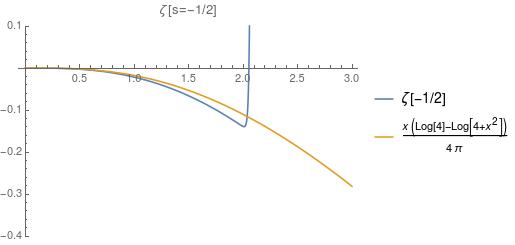
\includegraphics[scale=0.3]{Vacio.jpg}
    \caption{En esta imagen esta graficada la parte finita de la $\zeta _A (-1/2) $ en función del parámetro $x= \frac{\alpha}{x _0}$ donde se sumaron los primeros 100 términos de la serie, y en azul se puede ver la suma de la serie al reemplazar $\zeta (2n+1) = 1$}
    \label{fig:vacio}
\end{figure}























%\chapter{Extensiones Autoadjuntas del Operador}

    En Este capitulo se van a estudiar otras condiciones de contorno que hacen que el operador sea Autoadjunto en $x=0$ ademas de CC Dirichlet.

\section{Condiciones de Contorno Regulares}

En el capitulo anterior se estudiaron condiciones de contorno Dirichlet en ambos extremos, el objetivo de esta seccíon es ver si existen condiciones de contorno que en la ecuacion del espectro contengan $U(L)$ o su derivada

Suponiendo que en $x=0$ quiero poner las condiciones de contorno Robin mas generales:

\begin{equation}
\phi (0) + C \phi'(0) = 0 
\label{eq.robin}
\end{equation}

Los desarrollos de $U(x \rightarrow 0$ y $ F _1 ^1 (x \rightarrow 0 )$ están calculados en la ecuacion(REFERENCIAR) del capitulo anterior, puede verse que $F _1 ^1 (x)$ es una serie de potencia regular en $x=0$ entonces tanto $y_1 (x \rightarrow 0 ) \rightarrow 0$ como $y' _1 (x \rightarrow 0 ) \rightarrow 0$, como $U(x)$ posee potencias negativas y un termino logaritmico, $y _2 (x \rightarrow 0 ) \rightarrow Cte$ pero  $y' _2 (x \rightarrow 0 ) \rightarrow \infty $.

Para cualquier condicion de contorno de la forma (\ref{eq.robin} ) siempre obtengo $C[2] = 0$ entonces el espectro está dado por los ceros de $y[L]$ o $y'[L]$.


En la proxima seccion, voy a buscar extenciones autoajuntas del operador que puedna o no contener a $U(L)$ en el espectro.


\section{Artesanal}

Dado el Hamiltoniano $\mathscr{H} = - \partial ^2 _x + \frac{\alpha}{x}  $ voy a buscar condiciones de contorno que lo hagan autoadjunto en $x=0$ que es donde está la singularidad. 

La primer condicion necesaria es que su dominio e imagen pertenezcan a $L _2$.

\begin{equation}
\begin{array}{c}
si, \ \phi \in L _2 \rightarrow \mathscr{H} \phi \in L _2
\end{array}
\end{equation}


Como voy a estudiar el comportamiento en $x=0$, suponiendo que en $x=L$ todo es bien comportado, voy a empezar buscando soluciones analiticas en $x=0$, 

Basandome en el desarrollo de las autofunciones ( \ref{eq.scat} ) a  $x \rightarrow 0 $ 
Suponiendo que la primer funcion decae igual que la primer autofuncion $ y_1 (x) $.

\begin{equation}
\begin{array}{c}
\phi _1 (x \rightarrow 0) \approx x \ \rightarrow \phi _1 \ \in \ L _2 \\
\mathscr{H} [ \phi _1 ] (x \rightarrow 0) \approx \alpha \in L _2
\end{array}
\label{eq.chico1}
\end{equation}

Esto tambien vale para cualquier potencia positiva mayor 1, no vale para funciones que van a una constante debido a que el termino $1/x$ lo vuelve no integrable en el origen, luego se estudiara mas formalmente esta afirmacion.

Visto el comportamiento de la segunda autofuncion, propongo su comportamiento en $x \rightarrow 0 $ sea :

\begin{equation}
\begin{array}{c}
\phi _2 (x \rightarrow 0) \approx 1 + \alpha x Log[x] \\
\mathscr{H} [\phi _2] (x \rightarrow 0 ) \approx \alpha ^2 Log[x] \ \in L _2
\end{array}
\label{eq.chico2}
\end{equation}

Con estas propuestas dos funciones cualquiera en el dominio del operador tienen el desarrollo a $x \rightarrow 0$ :

\begin{equation}
\phi , \chi = \beta , \beta _1 \ x + \gamma , \gamma _1 \ (1+ \alpha x Log[x] )
\label{eq.phi.chi}
\end{equation}

La siguiente condicion es pedir que operador sea simetrico.

\begin{equation}
(\phi, \mathscr{H} \chi ) = ( \mathscr{H} \phi , \chi )
\end{equation}

Para ello voy a pedir que se anulen los terminos de borde

\begin{equation}
\begin{array}{c}
\int _0 ^{L} 
\left(
- \partial ^2 _x + \frac{\alpha}{x}
\right)
\phi ^{*} \chi dx = \\
\phi ^{*'} \chi - \phi \chi ^{* '} + 
\int _0 ^{L} 
\phi ^{*} 
| _{x=0} ^{x=L}
\left(
- \partial _x ^2 + \frac{\alpha}{x}
\right)
\chi dx 
\end{array}
\end{equation}

Suponiendo que $\phi $ y $ \chi $ ya satisfacen la condicion de contorno en $x=L$ e insertando el desarrollo de $\phi$ y $\chi$ dado por ( \ref{eq.phi.chi} ) , obtengo que para que el termino de borde se satisfaga debe cumplirse:

\begin{equation}
\left(
-1 + \alpha x 
\right)
\left(
\beta _1 ^{* '} \gamma - \beta \gamma _1 ^{* '}
\right)
\end{equation}

La cual se satiface si se cumple la doncidion 

\begin{equation}
\gamma = c \beta 
\end{equation}

Entonces toda funcion que esté en el dominio del operador va a tener un desarollo dado por:

\begin{equation}
\phi ( x \rightarrow 0 ) \approx x + c \left(  1 + \alpha x Log[x]   \right)
\end{equation}

Para cada $c$ que yo elija voy a obtener un Hamiltoniano con unas condiciones de contorno que lo vuelvan autoadjunto

\section{Teoria de Von Neumann}


Dado un operador diferencial de segundo orden $\mathscr{H}$ hay que definir cieras condiciones de contorno para que sea Hermitico.

Una forma de encontrar las condiciones de contorno que hacen que un operador sea hermitico (en el caso que estamos estudiando) es que las funciones del dominio se comporten en $x \rightarrow 0$ como:

\begin{equation}
\phi (x) \approx  A \phi (x) _{+} (x) + U(n) A \phi (x) _{-}
\end{equation}
 

Donde $|| \phi _{+/-} (x) || = 1$ y ambas son soluciones de 

\begin{equation}
\mathscr{H} \phi _{+/-} (x) = \pm i \phi _{+/-} (x)
\end{equation}

En general $U(n)$ que es el grupo unitario de orden n, es una isometria entre el las funciones $\phi _{+}$ y $\phi _{-} (x) $ pero como el problema a tratar tiene $n=1$ el unico elemento de $U(1) = e ^{i \gamma}$.


Como mi operador es real, basta hallar $\phi _{+} (x) $ y conjugarlo para hallar $ \phi _{-} (x) $, obtengo entonces 

\begin{equation}
\begin{array}{c}
\phi _{+} (x) = e ^{- \sqrt[4]{-1} x } e ^{i \sqrt{2} x } x . \\
\left(
F _1 ^1 (1 - \frac{ 4]{-1} }{2} \alpha ,2 , -2 (-1) ^{\frac{3}{4} } x )  +
U(1 - \frac{ \sqrt[4]{-1} }{2} \alpha ,2 , -2 (-1) ^{\frac{3}{4} } x )
\right)
\end{array}
\end{equation}

Para que satisfagan la condicion de contorno en $ x=L $ reescribo $ \phi _{+}$ como.

\begin{equation}
\phi _{+} (x) = \phi * _{-} (x) = 
= e ^{- \sqrt[4]{-1} x } e ^{i \sqrt{2} x } x.
\left(
F _1 ^1 (x=L) U(x) - U(x=L) F _1 ^1 (x)
\right)
\end{equation}


Utilizando (REFERENCIAR CAPITULO ANTEIOR), Los desarrollos quedan:

\begin{equation}
\begin{array}{c}
F _1 ^1 (x \rightarrow 0 ) \approx 1 \\
U( \rightarrow 0  ) \approx - \frac{1}{\alpha x \Gamma} + \frac{C}{\Gamma} + \frac{Log[x]}{\Gamma}
\end{array}
\end{equation}


Donnde $C$ es un numero complejo, insertando este desarrollo en (ARRIBA) y multiplicando por $ e ^{- i \gamma /2}$ obtengo:

\begin{equation}
\begin{array}{c} \\
\psi (x \rightarrow 0 )
A N ^{+}
\left(
-2 Re[ \frac{e ^{-i \gamma /2} F}{\alpha \Gamma} ] + 
2 x Re [ e ^{-i \gamma /2} (\frac{C F}{\Gamma} - U ) ] + 
2 x Log[x] Re [ e ^{- i \gamma /2 }]
\right)
\end{array}
\end{equation}

Lo cual luego de redefinir $C$ y $A$ queda 

\begin{equation}
\psi (x \rightarrow 0 ) = A N ^{+} 
\left(
x + C (1- \alpha Log[x] )
\right)
\end{equation}

Lo cual coincide con lo calculado anteriormente.

\section{Autofunciones:}

Las solcuciones de $H \phi (x) = \lambda ^2 \phi (x)$ ya fueron calculadas anteriormente 

\section{Funcion zeta}

El espectro de mi operador estará dado por los ceros de la funcion de onda en $x=L$

\begin{equation}
\begin{array}{c}
\frac{\psi (x=L)}{N L e ^{-i \lambda L} }
 = 
\left(
1+ i \lambda c - \alpha c 
\left(
2 \gamma -1 + Log[2 i \lambda] + 
\psi 
( 1 - \frac{i \alpha}{2 \lambda} )
\right)  
\right)
F _1 ^1 (1 - \frac{i \alpha}{2 \lambda},2,2 i \lambda L ) + \\
c \alpha \Gamma [-\frac{i \alpha}{2 \lambda}]
U (1 - \frac{i \alpha}{2 \lambda},2,2 i \lambda L )
\end{array}
\end{equation}

Para calcular la funcion $\zeta (s)$ voy a desarrollar en serie las funciones Hypergeometricas alrededor de $\lambda \rightarrow \infty$ para obtener:

\begin{equation}
\begin{array}{c}
\frac{(2 i \lambda L)}
{e ^{- \frac{\pi \alpha}{4 \lambda}}}
 \frac{\psi (x=L)}{N L e ^{-i \lambda L} } = 
 (- \alpha c Log[2 \lambda] + \lambda f[ \lambda ] ) 
 \left(
 \frac{e ^{  \frac{i \alpha Log[2 \lambda L ]}{2 \lambda } } e ^{2 i \lambda L } }
 {\Gamma ( 1 - \frac{i \alpha}{2 \lambda} )} S1 - 
 \frac{e ^{ -  \frac{i \alpha Log[2 \lambda L ]}{2 \lambda } } }
 	  {\Gamma (1 + \frac{i \alpha}{2 \lambda})} S2 
 \right) + \\
 c \alpha \Gamma (-\frac{i \alpha}{2 \lambda}) 
 e ^{- \frac{i \alpha Log[2 \lambda L]}{2 \lambda}} S2
\end{array}
\end{equation}

Donde $S1,S2$ y $f$ son series de potencias enteras negativas en $\lambda$ donde $S _{1,2} \rightarrow 1$ y $f \rightarrow i c$, cuando $\lambda \rightarrow \infty$.

Para calcular la funcion $zeta (s) $ voy a utilizar la integral en el plano complejo, trabajando con el lado derecho de la ecuacion , al igual que antes voy a tener un termino exponencialmente creciente/decreciente, dependiendo sobre que que eje me pare, obteniendo : 

\begin{equation}
\begin{array}{c}
Log[M[\lambda = i t]] = 
Log[S2] - 
\frac{i \alpha}{2 \lambda} Log[2 \lambda L] + % \\
Log[
	\frac{\alpha c Log[2 \lambda] - \lambda f[\lambda] }{\Gamma (1- \frac{i \alpha}{ 2 \lambda})} + 
	c \alpha \Gamma (- \frac{i \alpha}{2 \lambda}) ] \\ 
Log[M[\lambda = - i t]] = 
2 i \lambda L +
\frac{i \alpha Log[2 \lambda L]}{2 \lambda} -
Log[\Gamma (1- \frac{i \alpha}{2 \lambda}) ] +
Log[
	- \alpha c Log[2 \lambda] +
	\lambda f[\lambda]
	]
\end{array}
\end{equation}


Voy a empezar a analizar las contribuciones a los polos en $\lambda = i t$ \\

\textbf{Log[S2]:} \\

S2 es una serie de potencias que tiende a 1 en $\lambda \rightarrow \infty$, entonces tiene la forma:

\begin{equation}
S2 = 1 + \sum _{n=1} ^{\infty} \frac{a _n}{\lambda ^n}
\end{equation}

Su redivada Logaritmica la puedo escribir como es desarrollable y se puede escribir como:

\begin{equation}
\frac{S' [\lambda]}{1+ S[ \lambda ]} = \sum _{n=2} ^{\infty} \frac{b _n }{x ^n}
\end{equation}

De aquí se puede ver que este termino de la suma contribuira a polos simples, en los semienteros (como pasa en el problema regular) \\

$\mathbf{
- \frac{i \alpha}{2 \lambda} Log[2 \lambda L]} : 
$ \\

Este termino es el mismo que aparecía antes, y va a contribuir a un polo doble en $s=-1/2$  \\

$\mathbf{
Log[
	\frac{\alpha c Log[2 \lambda] - \lambda f[\lambda] }{\Gamma (1- \frac{i \alpha}{ 2 \lambda})} + 
	c \alpha \Gamma (- \frac{i \alpha}{2 \lambda}) ] :
}$ \\

Luego de desarrollar mi funcion $\Gamma$ se ve que dentro del Logaritmo hay 3 terminos que crecen indefinidamente:

\begin{equation}
\Gamma [- \frac{i \alpha}{2 \lambda}] = 
\frac{2 i \lambda}{\alpha} + 
\sum _{n=0} ^{\infty} \frac{c _n}{\lambda ^n}
\end{equation}

Sin embargo el termino dominante es orden $\lambda$, sacando factor comun $\lambda$ obtengo:

\begin{equation}
Log[\lambda] + 
Log \left[
	- \frac{1}{\Gamma[1- \frac{i \alpha}{2 \lambda}]} +
	2 i c -
	\left(
		\frac{\sum _{n=1} ^{\infty} \frac{f _n}{\lambda ^n}}
			 {\Gamma[1- \frac{i \alpha}{2 \lambda}]}		
		+ c \alpha \sum _{n=1} ^{\infty} \frac{c _n}{\lambda ^n} +
		\frac{\alpha c Log[2 \lambda]}{\lambda \Gamma [1 - \frac{i \alpha}{2 \lambda} ]}	
		\right)
		\right]		
\end{equation}


Donde toda la parte que está entre parentesis es infinitesimalmente chica, entonces voy a hacer un desarrollo alrededor del parentesis yendo a cero, (tambien se puede desarrollar la funcion $\Gamma$ que está abajo del 1, y poner todos los terminos que van a cero en el parentesis, pero el resultado final es el mismo)

\begin{equation}
Log[x + \epsilon] =
Log[x] + 
\sum _{n=1} ^{\infty}
	\frac{(-1) ^{1+n} }
     	{x ^n n}
     \epsilon ^{n}
\end{equation}

El termino 

\begin{equation}
Log[x] = 
Log \left[
		- \frac{1}{\Gamma [1 - \frac{i \alpha}{2 \lambda}]}
		\right] + 
2 i c
\end{equation}

Se comporta igual que el termino $ Log[S2] $, aquí lo nuevo vendrá de las potencias de $\epsilon$ \\
Vamos a analizar cada termino de la suma:

\begin{equation}
\frac{1}{x ^n} = 

\end{equation}




%\include{Capitulos/cap5}
\thispagestyle{empty}
\chapter{Conclusiones}

A lo largo de este trabajo de tesis se estudió la energía de vacío asociada al operador singular $A = - \partial ^2 _x + \frac{\alpha}{x} $ para lo cual se analizaron los polos de su correspondiente función-$\zeta$.

En los capítulos \ref{cap.singular} y \ref{cap.continuo} se tomaron como dominio del operador los intervalos compacto $[0,L]$ y no compacto $[0, \infty)$ respectivamente, en ambos casos se obtuvo un polo simple en $s = \frac{1}{2}$ cuyo residuo está dado por
\begin{equation}
{\rm Res } \ \zeta (s) \big|_{s = \frac{1}{2}}
= \frac{L \mu}{2 \pi} 
= \frac{ {\rm Vol (\mathcal{M})} }{2 \pi} 
\, ,
\end{equation}
donde $\mathcal{M}$ es el volumen de la variedad, este resultado coincide con el presentado en \eqref{eq.vol}, lo cual es importante ya que el operador bajo estudio no cumple con las condiciones requeridas para que su Heat Kernel posea un desarrollo de la forma \eqref{eq.heat.expansion}, lo que abre el interrogante sobre la posible extensión del resultado \eqref{eq.vol} en operadores singulares.



En cuanto al estudio de $\zeta (s= -\frac{1}{2} )$, término presente en la definición de la Energía de Casimir \eqref{e0-zeta}, en ambos casos (intervalo compacto y no compacto) se demostró que tal como ocurre en $s= \frac{1}{2}$ el polo es independiente del intervalo pero a diferencia del caso regular se encontró que posee un polo doble dado por
\begin{align*}
&
	\zeta \left( - \frac{1}{2} + \epsilon \right) = 
	\frac{\alpha}{8 \pi \mu  \epsilon  ^2} +
	\frac{\alpha \left( \log (2 L \mu ) + \gamma -1  \right)}{4 \pi \mu  \epsilon } +
	{\rm PF } \zeta \left( - \frac{1}{2} \right)
\, ,
\end{align*}
lo que demuestra que el desarrollo asintótico del Heat-Kernel presenta términos logaritmicos. 
% tal como se conjeturó en 1980 \cite{callias1980}.


En cuanto al estudio de los demas polos se concluyó que al igual que en el caso regular son todos simples y están ubicados en los semienteros negativos. Utilizando este resultado y el anterior se confirma la conjetura dada en \cite{callias1980} la cual afirma que el Heat-Kernel para operadores singulares posee un desarrollo de la forma  
\begin{equation}
	K(T) \sim 
	\frac{ \log (T)}{T ^{\frac{1}{2} }} C _{2} +
	\sum _{\substack{n=0 \\ n \neq 2}} ^{\infty}
	C _n  \ 
	T^{\frac{(-1+n)}{2}} 
\, ,
\end{equation}
este resultado es muy importante ya que exceptuando el polo en $s = - \frac{1}{2}$ el desarrollo del Heat-Kernel coincide en estructura con el caso regular lo cual no se cumple para otros operadores singulares, un ejemplo de esto es el operador $- \partial ^2 _x + \frac{\alpha}{x ^2}$ en donde se demostró que sus polos pueden caer incluso valores irracionales \cite{doi:10.1063/1.1809257}.


En cuanto al estudio de la parte finita de $\zeta \left( - \frac{1}{2} \right)$ se obtuvieron dos representaciónes, una integral y un desarrollo en serie, dependientes del parámetro adimensional $\beta = \alpha L$, a partir de la cual se generaron curvas de la energía de vacío para distintos valores de $\alpha$ y $L$, se observó que la energía de vacío posee en máximo local en el cual para  $L < L _{critico} $ la fuerza es atractiva y luego se recupera el clásico comportamiento repulsivo, comportamiento también presente en potenciales regulares \cite{Beauregard_2013}.\\

Dado que la energía de casimir depende profundamente de la geometría se a utilizado ampliamente en distintos modelos, en \cite{Blau_1988} se mencionan algunas aplicaciones como por ejemplo, las placas paralelas neutras en el vacio \cite{PLUNIEN198687}, dinamica de campos sobre membranas en teoría $M$ \cite{DEWIT1988545}, modelos de quarks en el nucleo atómico \cite{PhysRevD.14.2622}, etc. En partícular un modelo que se cita es una aproximación semi-clasica de la estructura del electrón \cite{MILTON198049} en el cual se propone un modelo de electrón formado por un cascaron esferico que se mantiene estable debido a un equilibrio entre la  energía electrostática repulsiva y la energía de casimir atractiva del campo en el interior del cascaron.

Inspirado en este último ejemplo se pueden proponer dos interpretaciones, la primera está relacionada con el trabajo original de Casimir \cite{Casimir:1948dh}, en el cual el sistema está formado por dos placas paralelas en el vacío donde una está cargada de tal forma que genera un pontencial electrostático $V (x) = \frac{\alpha}{x}$, en esta interpretación la energía de casimir calculada corresponde a la energía por unidad de area tal como se explica en \cite{Blau_1988}.

La segunda interpretación posible está inspirada en \cite{MILTON198049} y \cite{Beauregard_2013}, donde en vez de pensar que dos placas paralelas interactuan en el vacío, el sistema son dos partículas de igual carga sometidas a su campo electromanético, lo cual para $L _{critico} < L$ genera una fuerza repulsiva como es de esperar, pero a partir de un valor límite $L < L _{critico}$ las partíclas sufren una fuerza atractiva.












\thispagestyle{empty}


%----------------------------------------------------------------------------------------
%	APÉNDICES
%----------------------------------------------------------------------------------------

%\addtocontents{toc}{\vspace{1cm}} 
% Agrega espacios en la toc pero de manera rara

\appendix % Los siguientes capítulos son apéndices

%Incluye los apéndices en el folder de apéndices

\chapter{Calculo de las correciones asintoticas la Funcion Hypergeometrica}

n el capitulo 3, cuando se calcularon asintoticamente los autovalores, se utilizo la aproximacion:  

\begin{equation}
    F _1 ^1 (a,b,z) = \Gamma (b) 
    \left(
    \frac{e^z z ^{a-b} }{\Gamma(a)} * A_1 + \frac{(-z) ^{ -a}}{ \Gamma(b-a)} 
    * A_2
    \right)
\end{equation}

Donde $A_1$ y $A_2$ quedan determinadas por:

\begin{equation}
\begin{array}{c}
    A _1 = 
    \sum _{n=0} ^{R-1} 
    \left(
    \frac{(a) _n (1+a-b) _n}{n!} (-z) ^{-n} + O(|z| ^{-R})
    \right) \\
    A _2 = 
    \sum _{n=0} ^{S-1} 
    \left(
    \frac{(b-a) _n (1-a) _n }{n!} z ^{-n} + O(|z| ^{-s})
    \right)
\end{array}
\end{equation}

Donde $(a)_ n$ es el símbolo de Pochhammer, las primeras correcciones en $A_1$ y $A_2$ quedan,Luego de reemplazar $a,b,z$ por sus valores:

\begin{equation}
\begin{array}{c}
    A _1 = 1 + \frac{a(1-a-b)}{-z} + O(|z| ^ {-2})
    =  - \frac{\beta}{4 \mu ^2} + \frac{\beta ^2}{8 i \mu ^3} + O(|\mu| ^{-3}) \\ 
    A _2 = 1 + \frac{(b-a)(1-a)}{z} + O(|z| ^{-2}) = 
    - \frac{\beta ^2}{8 i \mu ^3} - \frac{\beta}{4 \mu ^2} + 
    O(|\mu| ^{-3})
\end{array}
\end{equation}

De aquí puede verse que la primer corrección asintótica entra al orden mas bajo en la potencia $\mu ^2$, que no contribuye al polo en $s= -1/2$ ya que la ecuación asintótica, el del orden $\frac{1}{\mu ^2}$ cuando quiero calcular el polo en $s=-3/2$.

\chapter{Función-$\zeta$ de Riemman}\label{Apendice.2}

En este apéndice se demostraran las propiedades de la función-$\zeta$ de Riemman $\zeta _R (s)$

La función $\zeta _R (s)$ se define como la prolongación analítica de la siguiente serie
\begin{align}
	\zeta _R (s) = 
	\sum _{n=1} ^{\infty} \frac{1}{n ^{s}}
	\, ,
\end{align}
para calcular sus propiedades se utilizará la identidad
\begin{align}
	\frac{1}{n ^{s}} =
	\frac{1}{\Gamma (s)} 
	\int _0 ^{\infty} t^{s-1} e ^{-n t}  dt
	\, ,
\end{align}
obteniendo
\begin{align}
	\zeta (s) = 
	\frac{1}{\Gamma (s)}
	\int _0 ^\infty
	\frac{t ^{s-1}}{e ^t -1} dt
	\, ,
\end{align}
aquí puede utilizarse el desarrollo de taylor 
\begin{equation}
	\frac{1}{e ^t -1} = 
	\sum _{n=-1} ^{\infty}
	\frac{ \mathcal{B} _{n+1}}{(n+1)!} t ^n
	\, ,
\end{equation}
donde $\mathcal{B} _{n}$ son los {\it Números de Bernoulli}, utilizando esta representación $\zeta (s)$ queda expresada como
\begin{align}
	\zeta (s) = 
&
	\frac{1}{\Gamma (s)}
	\int _0 ^1 
	t ^{s-1} 
	\left(	
		\frac{1}{e ^t -1} -
		\sum _{n=-1} ^{N}
		\frac{ \mathcal{B} _{n+1}}{(n+1)!} t ^n	
		\right)		
		+
	\frac{1}{\Gamma (s)}
	\int _1 ^\infty
	\frac{t ^{s-1}}{e ^t -1} dt
\\
	+
&
	\frac{1}{\Gamma (s)}
	\sum _{n=-1} ^{N}
	\frac{ \mathcal{B} _{n+1}}{ (n+1)! (n + s)}
	\, ,
\end{align}
así $\zeta (s)$ podrá ser calculada $\forall s $ en algún lado, dos valores característicos de $\zeta(s)$ están dados por
\begin{align}
	\zeta (-1) = 
&
	Res \Big| _{s=1}
		\left(
			\frac{1}{\Gamma (s)} \frac{\mathcal{B} _2}{2! (s+1)}
			\right) =
	- \frac{1}{12}
\\
	\zeta (\epsilon \rightarrow 1) =
& 
	\frac{1}{\Gamma (1)} \frac{\mathcal{B} _0}{ \epsilon} + O (\epsilon -1 ) = 
	\frac{1}{ \epsilon} + O (\epsilon -1 ) 
	\, ,
\end{align}
otra propiedad importante es la no existencia de polos exceptuando $s=1$, para esto se ve que la única posible contribución a un polo son los términos de la forma  $	\frac{1}{\Gamma (s)} \frac{ \mathcal{B} _{n+1}}{ (n+1)! (n + s)}$, para esto 
\begin{align}
	\zeta ( s \rightarrow -n ) = 
	\frac{1}{\Gamma (s)}
	\frac{ \mathcal{B} _{n+1}}{ (n+1)! (n + s)}
	+ O (s + n) = 
	\frac{(-1) ^n \mathcal{B} _{n+1}}
		{n+1}
\end{align}























\chapter{Otras condiciones de contorno}\label{Apendice.3}



En este apéndice se demostrará que el operador \ref{operador} solamente admite condiciones de contorno Dirichlet en ambos extremos
\begin{equation}
A = - \partial ^2 _x + \frac{\alpha}{x}
\end{equation}





\thispagestyle{empty}


%\addtocontents{toc}{\vspace{2cm}} % Agrega espacio en la toc


%----------------------------------------------------------------------------------------
%	BIBLIOGRAFÍA
%----------------------------------------------------------------------------------------
\backmatter
\nocite{*}
\bibliographystyle{plain}
\bibliography{bib.bib} %Aquí ponen el nombre del archivo .bib


\end{document}